\documentclass[master=cws,masteroption=ai,english]{kulemt}
\setup{title={Learning Constraints and Optimization Criteria},
  author={Samuel Kolb},
  promotor={Prof.\,dr.\ Luc De Raedt \and Dr. ir.\ Anton Dries},
  assessor={Dr. Jan Tobias M\"uhlberg},
  assistant={}}

% The following \setup may be removed entirely if no filing card is wanted
\setup{filingcard, translatedtitle={Het leren van beperkingen en optimalisatie criteria}, udc={681.3*I20}, shortabstract={Deze thesis presenteert een leersysteem voor beperkingen en een leersysteem voor optimalisatie criteria.
Beperking worden geleerd in de vorm van clausules in eerste orde logica door het gebruik van ILP technieken.
Voor de optimalisatie criteria wordt het gebruik van gewogen clausules voorgesteld.
Beide systemen zijn in staat om essenti\"ele beperkingen en optimalisatie criteria te leren.
De invloed van verschillende interne en externe factoren wordt onderzocht.
Er wordt een procedure voorgesteld om de gewogen clausules in eerste orde logica te gebruiken om optimale oplossingen te vinden.\\\\This thesis presents two systems that are able to automatically learn constraints from examples and optimization criteria from rankings, respectively.
Both hard and soft constraints can be learned and constraints are represented as first order logical clauses.
Choosing such clauses as representations enables the use of ILP techniques such as clausal discovery.
In this research optimization criteria are represented as weighted clauses.
Several experiments show that both systems are able to achieve their tasks.
The impact of various internal and external factors is experimentally tested to provide insights into the way they influence the learning systems.
For all examples, the clause learning system could find the essential constraints.
The learning system for optimization criteria is shown to achieve accurate results and can learn criteria that identify the correct optimal solution even for few examples and noisy rankings.
Finally, a procedure is outlined that allows weighted first order logic clauses to be used for optimization.
}}
% Uncomment the next line for generating the cover page
% \setup{coverpageonly}
% Uncomment the next \setup to generate only the first pages (e.g., if you
% are a Word user.
%\setup{frontpagesonly}

% Choose the main text font (e.g., Latin Modern)
\setup{font=lm}

% If you want to include other LaTeX packages, do it here. 
\usepackage{algorithm}
\usepackage{algpseudocode}
\usepackage{amsmath}
\usepackage{amssymb}
\usepackage{amsthm}
\usepackage{etoolbox}
\usepackage{changepage}
\usepackage{csquotes}
\usepackage{tabularx,booktabs,multirow}
\usepackage{longtable}
\usepackage{framed}
\usepackage{breakcites}
\usepackage{listings}
\usepackage{pdfpages}

\lstset{
    frame=single,
    breaklines=true,
    postbreak=\raisebox{0ex}[0ex][0ex]{\ensuremath{\color{black}\hookrightarrow\space}}
}


\graphicspath{{Graphics/}, {Graphics/Graphs/}{Paper/Graphics/}}

\newcommand{\sym}[1]{\ensuremath{\mathcal{#1}}}
\newcommand{\obj}[1]{\ensuremath{#1}}

\newtheorem{definition}{Definition}[chapter]
\newtheorem{question}{Question}
\AfterEndEnvironment{definition}{\noindent\ignorespaces}

\theoremstyle{definition}
\newtheorem{example}{Example}[chapter]
\newtheorem{experiment}{Experiment}[question]
\newtheorem{observation}{Observation}[question]
%\AfterEndEnvironment{example}{\noindent\ignorespaces}

\newcommand{\svm}{SVM$^{rank}$}
\newcommand{\cen}[1]{
	\begin{center}
		#1
	\end{center}
}

\newenvironment{demo}{\begin{adjustwidth}{2cm}{}}{\end{adjustwidth}}

\makeatletter
\newenvironment{shiftedflalign}{%
    \start@align\tw@\st@rredfalse\m@ne%
    \hskip\parindent
}{%
    \endalign
}
\newenvironment{shiftedflalign*}{%
    \start@align\tw@\st@rredtrue\m@ne
    \hskip\parindent
}{%
    \endalign
}
\makeatother

\newcommand{\tabspace}{\  \  \  \  }

% Finally the hyperref package is used for pdf files.
% This can be commented out for printed versions.
%\usepackage[pdfusetitle,colorlinks,plainpages=false]{hyperref}
\usepackage[pdfusetitle,plainpages=false]{hyperref}

%\includeonly{chap-n}
\begin{document}

\begin{preface}
I thank my promoter Prof. dr. Luc de Raedt, who has inspired me throughout my academic career and never hesitated to provide his help and guidance in these years.
\\\\
I thank my promoter and daily supervisor Dr. ir. Anton Dries, who has always been available for me, even on short notice.
\\\\
Furthermore, I express my gratitude for the technical assistance and insights provided by Bart Bogaerts, Prof. dr. Jesse Davis, Prof. dr. Marc Denecker en Vladimir Dzyuba.
\\\\
I would also like to acknowledge some of the people that are close to me and have provided me with direct or indirect help during the completion of my thesis:
A big thank you to my girlfriend An, for her continuous support and her corrections.
I thank my friends Anna and Glenn for providing me with helpful corrections during the writing process.
Last, but not least, thank you Helena, Roxane and Wolfgang for supporting me in all my endeavors.
\end{preface}

\tableofcontents*

\begin{abstract}
This thesis presents two systems that are able to automatically learn constraints from examples and optimization criteria from rankings, respectively.
Both hard and soft constraints can be learned and constraints are represented as first order logical clauses.
Choosing such clauses as representations enables the use of ILP techniques such as clausal discovery.
In this research optimization criteria are represented as weighted clauses.
Several experiments show that both systems are able to achieve their tasks.
The impact of various internal and external factors is experimentally tested to provide insights into the way they influence the learning systems.
For all examples, the clause learning system could find the essential constraints.
The learning system for optimization criteria is shown to achieve accurate results and can learn criteria that identify the correct optimal solution even for few examples and noisy rankings.
Finally, a procedure is outlined that allows weighted first order logic clauses to be used for optimization.
\end{abstract}

\begin{abstract*}

\textit{Deze samenvatting komt overeen met het artikel dat te vinden is in appendix~\ref{app:article}}.

\paragraph{Abstract}
Deze thesis presenteert een leersysteem voor beperkingen en een leersysteem voor optimalisatie criteria.
Beperking worden geleerd in de vorm van clausules in eerste orde logica door het gebruik van ILP technieken.
Voor de optimalisatie criteria wordt het gebruik van gewogen clausules voorgesteld.
Beide systemen zijn in staat om essenti\"ele beperkingen en optimalisatie criteria te leren.
De invloed van verschillende interne en externe factoren wordt onderzocht.
Er wordt een procedure voorgesteld om de gewogen clausules in eerste orde logica te gebruiken om optimale oplossingen te vinden.
%!TEX root=Paper.tex
\section{Introductie}
% no \IEEEPARstart
% You must have at least 2 lines in the paragraph with the drop letter
% (should never be an issue)

Computers worden veelal gebruikt voor het oplossen van problemen die handmatig maar moeilijk opgelost kunnen worden. 
Hiervoor worden klassiek computerprogramma's gebruikt.
Dit zijn essentieel stap-voor-stap instructies die beschrijven hoe een probleem opgelost moet worden.
Als alternatief voor dit soort \emph{imperatief} programmeren kunnen problemen beschreven worden op een \emph{declaratieve} manier.
Hierbij ligt de focus op het formuleren van het probleem op een hoog niveau.
Zo een taal beschrijft het probleem zonder in te vullen hoe een oplossing gevonden moet worden.
Voor deze talen worden generische algoritmes ontworpen die automatisch oplossingen kunnen zoeken.

Een populaire stroming binnen het veld van declaratief programmeren is constraint programming.
In constraint programming worden variabelen gebruikt om problemen voor te stellen.
Elke variabele heeft een domein en er worden beperkingen (constraints) opgelegd aan de waarden van de variabelen.
De constraint solver zal proberen elke variabele een waarde uit zijn domein toe te kennen zodanig dat alle beperkingen voldaan zijn.
Hierbij focust de gebruiker op het opstellen van de beperkingen en kan de solver zelf kiezen op welke manier oplossingen gevonden kunnen worden.

Constraint programming is niet enkel populair binnen de academische wereld, het wordt ook succesvol gebruikt in de industrie\cite{Simonis:IndustrialApplicationsCP}.
De meeste aandacht wordt besteed aan het verbeteren van solvers, maar het blijkt in de praktijk best moeilijk voor niet-deskundigen om beperkingen te formuleren\cite{Wallace:PrinciplesCP}.

Het eerste doel van dit onderzoek is het automatiseren van het opstellen van beperkingen.
Door deze beperkingen te leren met behulp van enkele voorbeelden, probeert dit werk om onder andere het programmeren met beperkingen toegankelijker te maken.

Beperkingen zullen worden uitgedrukt door logische clausules (clauses).
Deze laten toe om technieken uit het veld van inductief logisch programmeren (ILP) te gebruiken.
Specifiek, wordt een nieuwe implementatie van het clausal discovery algoritme\cite{DeRaedt:ClausalDiscovery} uitgewerkt.
Onderzoek naar technieken voor het leren van beperkingen loopt vaak onafhankelijk van de ontwikkelingen in ILP.
Dit onderzoek knoopt aan bij het idee van Lallouet et al.\cite{Lallouet:LearningCP} om voor deze taak ILP technieken te gebruiken.
\\\\
Harde beperkingen kunnen gebruikt worden om oplossingen te onderscheiden van niet-oplossingen.
Zogenaamde zachte beperkingen (soft constraints) kunnen eigenschappen uitdrukken die niet voldaan hoeven te zijn.
Door aan zulke beperkingen gewichten te geven kan het belang van dergelijke beperkingen uitgedrukt worden.
Dit laat toe om binnen de toelaatbare oplossingen een optimale oplossing te vinden.
Deze oplossing voldoet aan zo veel mogelijk belangrijke beperkingen.

Het tweede doel van dit onderzoek omvat het leren van de voorkeuren van een gebruiker en het formuleren van overeenkomstige optimalisatie criteria.
Door middel van rangschikkingen van een aantal voorbeelden worden gewogen zachte beperkingen opgesteld.
Dit moet, zoals het leren van beperkingen, de kloof tussen problemen en formele representaties verkleinen.

Het gebruik van gewogen zachte beperkingen is onder andere ge\"inspireerd door het onderzoek van Campigotto et al.\cite{campigotto2011active}.
Hierin wordt een gelijkaardige doelstelling onderzocht in een interactieve context voor propositionele beperkingen.
In dit onderzoek zullen beperkingen in eerste orde logica worden gebruikt.
\\\\
Het volledige proces van probleem naar oplossing vergt ook een solver voor het automatisch vinden van een oplossing.
Voor de gewogen beperkingen die door dit systeem geleerd worden bestaat er geen solver die deze representatie direct kan gebruiken.
Daarom zal worden aangetoond hoe deze beperkingen in de praktijk gebruikt kunnen worden om een optimale oplossing te vinden.

% ----------------------------------------
% Achtergrond
% ----------------------------------------

\section{Achtergrond}
Deze sectie geeft een bondig overzicht over gebuikte concepten en relevante literatuur.

\subsection{Clausules}
Clausules in eerste orde logica zijn disjuncties van literalen.
Een literaal is gedefinieerd als een atoom of de negatie van een atoom.
Vaak worden clausules uitgedrukt door middel van een lichaam (body) en hoofd (head): $\mathit{hoofd} \leftarrow \mathit{lichaam}$.
Alle literalen met een negatie worden gegroepeerd in het lichaam en en de anderen in het hoofd.
\begin{align*}
  \lnot a_1 \lor \lnot a_2 \lor a_3 \lor a_4 = a_3, a_4 \leftarrow a_1, a_2 
\end{align*}

Atomen zijn logische concepten waaraan een waarheidswaarde kan worden toegekend.
In dit onderzoek zijn atomen beperkt tot predicaten.
Een predicaat bevat een predicaat symbool en een aantal termen.
Die termen zijn constanten of variabelen en beschrijven objecten in een domein.
Predicaten drukken relaties uit tussen die objecten: $\mathit{symbool}(\mathit{term_1}, ... \mathit{term_n})$.
De clausules die in dit onderzoek geleerd worden bevatten enkel variabelen.

\subsection{Leren van beperkingen}
Het leren van beperkingen is een moeilijk probleem.
De zoekruimte om beperkingen te vinden is vaak erg groot.
Bovendien zijn er, in tegenstelling tot veel problemen binnen het veld van machinaal leren, meestal weinig voorbeelden gegeven om van te leren.

Verschillende systemen proberen het leren van beperkingen op verschillende manieren op te lossen.
Een manier om het probleem van weinig data op te lossen is om data interactief te genereren.
De systemen Conacq2\cite{bessiere2007query} en QuAck\cite{bessiere2013constraint} genereren voorbeelden en vragen aan de gebruiker om deze al dan niet goed te keuren.

In een passieve setting probeert ModelSeeker\cite{Beldiceanu:ModelSeeker} de probleem variabelen op verschillende manieren te structureren.
Daaraan wordt getest of dat bepaalde algemene beperkingen gelden binnen deze structuren.
Deze manier laat toe om effici\"ent beperkingen te leren van maar enkele voorbeelden.

Zoals vermeld werd in de inleiding werd in het onderzoek van Lallouet et al.\cite{Lallouet:LearningCP} ook al geprobeerd om ILP technieken te gebruiken voor het leren van beperkingen.
Hierbij wordt de zoekruimte van mogelijke beperkingen op een bidirectionele manier doorzocht waarbij vooral negatieve voorbeelden gebruikt worden.

\begin{algorithm}
  \caption{Clausal discovery algoritme}
  \label{alg:cd_alg}

  \begin{algorithmic}
  \State $\sym{D} \gets Examples$
  \State $Q \gets \{\square\}$
  \State $\sym{T} \gets \{\}$
  \While{$\lnot isempty(Q)$}
    \State $c \gets next(Q)$
    \If{$covers(c, \sym{D})$}
      \If{$\lnot entails(\sym{T}, c)$}
        \State $\sym{T} = \sym{T} \cup c$
      \EndIf
    \Else
      \State $Q \gets Q \cup \rho(c)$
    \EndIf
  \EndWhile
  \State $\sym{T} \gets prune(\sym{T})$
  \State \Return \sym{T}
\end{algorithmic}
\end{algorithm}

In dit onderzoek werd er vooral gekeken naar clausal discovery\cite{DeRaedt:ClausalDiscovery}.
Het algoritme~\ref{alg:cd_alg} werd voorgesteld om vooral op basis van positieve voorbeelden logische clausules te leren.
Dit algoritme bevat bepaalde conceptuele functies zoals $\mathit{covers}, \mathit{entails}$ en $\rho$.
Het systeem dat in dit onderzoek ontwikkeld werd gebruikt deze functies maar vult deze anders in.
Om te berekenen of een clausule waar is voor de voorbeelden in een dataset ($\mathit{covers}$) en of een nieuwe clausule een logisch gevolg is van de reeds gevonden clausules ($\mathit{entails}$) wordt een logisch systeem gebruikt.
De functie $\rho$ wordt de \textit{refinement operator} genoemd.
Deze produceert verschillende mogelijke uitbreidingen van een clausule.
Elke uitbreiding wordt verkregen door een literaal toe te voegen aan de gegeven clausule.
Zodanig wordt, vertrekkende van de lege clausule~($\square$), de zoekruimte verkend door clausules steeds algemener te maken.

\subsection{Logische solver}
Dit onderzoek gebruikt het logisch systeem IDP\cite{de2013prototype,wittocx2008idp} om de functies $\mathit{convers}$ en $\mathit{entails}$ te berekenen.
Het systeem laat toe om oplossingen te verifi\"eren maar ook te genereren.
IDP ondersteunt een uitbreiding van eerste orde logica: $FO(\cdot)$.
Achtergrondkennis van een gebruiker over de gebruikte predicaten kan in dit formaat worden meegegeven.

\subsection{Optimalisatie}
De vraag of er aan een propositionele logische formule voldaan kan worden wordt het vervulbaarheidsprobleem (SAT) genoemd.
Een uitbreiding hiervan is het MAX-SAT probleem.
Hierin wordt geprobeerd om in een formule in conjunctieve normaalvorm (CNF) zoveel mogelijk clausules (disjuncties) waar te maken.
Als aan die clauses een gewicht wordt toegekend bekomt men het gewogen MAX-SAT probleem.
In Campigotto et al.\cite{campigotto2011active} werd het automatische leren van propositionele formules en gewichten onderzocht.
Ge\"inspireerd door hun resultaten zullen in dit onderzoek eerste orde logische optimalisatie criteria gezocht worden.
Het optimalisatie vraagstuk kan dan gezien worden als een uitbreiding van gewogen MAX-SAT waarbij de clausules in eerste orde logica zijn.

% ----------------------------------------
% Probleemstelling
% ----------------------------------------

\section{Probleemstelling}
Dit onderzoekt heeft hoofdzakelijk twee doelen: het leren van beperkingen en het leren van optimalisatie technieken.
De systemen die in de context van deze doelstellingen ontworpen worden proberen het opstellen van formele representaties te vereenvoudigen.
Om de software toegankelijk te maken wordt er aandacht besteed aan de informatie die van de gebruiker gevraagd wordt.

\begin{framed}
  \noindent
  \begin{minipage}{\textwidth}
    \paragraph*{Doel 1}
    Gegeven een aantal voorbeelden en een limiet $t$ is het doel van het leersysteem voor beperkingen om zo specifiek mogelijke clausules te vinden die door ten minste $t$ van de gegeven voorbeelden voldaan worden.
  \end{minipage}
\end{framed}

Voorbeelden beschrijven specifieke oplossingen.
Ze bevatten een set objecten en beschrijven exhaustief alle relaties (predicaten) die van toepassing zijn op deze objecten.
De geleerde clausules zijn onafhankelijk van de specifieke objecten in de voorbeelden en bevatten enkel variabelen.

\begin{framed}
  \noindent
  \begin{minipage}{\textwidth}
    \paragraph*{Doel 2}
    Gegeven een aantal voorbeelden en een aantal rangschikkingen over deze voorbeelden is het doel van het leersysteem voor optimalisatie criteria om zachte beperkingen en gewichten te vinden, zodanig dat de orde die door deze criteria beschreven wordt optimaal overeenkomt met de gegeven rangschikkingen.
  \end{minipage}
\end{framed}

De zachte beperkingen zijn clausules die op sommige van de voorbeelden gelden.
Rangschikkingen zijn van het formaat: $e_x = e_y > ... > e_a = e_b$ en beschrijven telkens een parti\"ele orde.
Door middel van de gewogen clausules kan voor elk voorbeeld een score berekend worden.
\begin{align*}
  \sum\limits_{\mathit{gewicht}, \mathit{c}} \mathit{gewicht} \cdot v_{c}
\end{align*}
Indien de clausule voldaan is voor het voorbeeld is de term $v_c = 1$, anders is $v_c = 0$.
Met behulp van deze scores kan een totale orde gedefinieerd worden over de voorbeelden.
\\\\
Een derde doel van deze thesis is om aan te tonen hoe deze beperkingen en vooral de optimalisatie criteria in de praktijk gebruikt kunnen worden om een optimale oplossing te vinden.

% ----------------------------------------
% Aanpak
% ----------------------------------------

\section{Aanpak}
Voor dit onderzoek werd een implementatie gecre\"eerd van een leersysteem voor clausules en een leersysteem voor gewogen clausules.
Figuur~\ref{fig:struktuur} toont een overzicht.
Clausules worden geleerd met behulp van voorbeelden.
Om gewogen clausules te vinden wordt eerst behulp gemaakt van het leersysteem van clausules om zachte beperkingen te vinden.
Daarna worden gewichten voor deze beperkingen bepaald op basis van de rangschikkingen.
Dit gebeurt met behulp van de \svm software.

\begin{figure}

  \centering
    \includegraphics[width=1\linewidth]{AanpakOverzicht.pdf}
  \caption{Overzicht aanpak}
  \label{fig:struktuur}

\end{figure}

\subsection{Formaat}
De voorbeelden worden gegroepeerd in een bestand.
In het begin van het bestand volgen een aantal definities van types en predicaten.
Types zijn een vorm van kennis die een gebruiker vaak heeft en die de nauwkeurigheid en effici\"entie van het systeem ten goede komt.
Definities van predicaten beschrijven wat voor types de termen van dat predicaat moeten hebben.
Twee speciale vormen van predicaten zijn toegelaten: berekende predicaten en symmetrische predicaten.
Voor berekende predicaten wordt in de achtergrondkennis gespecificeerd hoe ze berekend moeten worden.
Deze predicaten worden dus niet expliciet gegeven in de voorbeelden.
Symmetrische predicaten zijn predicaten waarbij de volgorde van de predicaten niet uitmaakt.

\subsection{Clausal discovery}
Het leersysteem voor clausules is, zoals eerder vernoemd, gebaseerd op clausal discovery.
Voor de essenti\"ele functies $\mathit{covers}$ en $\mathit{entails}$ wordt het logisch systeem IDP gebruikt.
IDP gebruikt vier componenten: een vocabularium van types en definities, theorie\"en van formules, structuren en een procedure.
Het vocabularium kan worden gegenereerd vanuit de definities en structuren.
Voorbeelden kunnen gezien worden als structuren, maar structuren moeten niet volledig gespecificeerd zijn.
De procedure wordt gebruikt om verschillende soorten inferenties uit te voeren over de theorie\"en en structuren.
Voorbeelden zijn het verifi\"eren of het het vervolledigen van een structuur gegeven een theorie.

Als een clausule in de wachtrij geplaatst wordt zullen de nodige IDP componenten gegenereerd worden om de $\mathit{covers}$ test uit te voeren.
Zodra de clausule uit de wachtrij genomen wordt, worden twee tests uitgevoerd.
De subset-test bepaalt of dat de clausule een super set is van een andere clausule die eerder al geaccepteerd werd.
Indien dat zo is en de andere clausule voor dezelfde voorbeelden geldt, dan is de nieuwe clausule onnodig.
Anders zal getest worden of dat de clausule zelf voor genoeg voorbeelden voldaan is.
Indien ja, zo wordt zij geaccepteerd en mogelijks als beperking aanvaard, anders wordt de clausule uitgebreid door $\rho$.
Een geaccepteerde clausule kan redundant zijn als ze een logisch gevolg is van de achtergrond kennis en de reeds gevonden beperkingen.
Dit wordt achterhaald door de $\mathit{entails}$ functie, gebruikmakende van IDP.

Een belangrijke stap is het uitbreiden van clausules.
Op basis van het maximum aantal variabelen wordt op voorhand een lijst~$L$ opgesteld van atomen die kunnen worden toegevoegd aan een clausule.
Binnen het lichaam en hoofd van de clausule mogen deze atomen enkel in de juiste volgorde worden toegevoegd.
Bovendien moet er voldaan worden aan de types van de predicaten en zijn er restricties op het formaat van de clausules.
Clausules moeten \emph{verbonden} (connected) zijn.
Voor verbonden clausules is het onmogelijk om de literalen in twee delen op te splitsen zodanig dat geen enkele variabele voorkomt in beide delen.
Een tweede restrictie is dat de variabelen die voorkomen in het hoofd van de clausule ook moeten voorkomen in het lichaam (range-restricted).
Vaak kunnen clausules op verschillende manieren herschreven worden.
Het is enkel nodig om een van die vormen te genereren.
Door te kijken naar de posities van de atomen van de clausule in de lijst~$L$ kan een kleinste equivalente clausule bepaald worden.
Deze clausule wordt de vertegenwoordiger genoemd en enkel clausules in deze vorm worden als uitbreidingen toegelaten.

\subsection{Optimalisatie}
Voor het leren van optimalisatie criteria worden eerst zachte beperkingen gezocht met behulp van het vorige leersysteem.
Hiervoor wordt een lage limiet opgegeven, in het standaard geval is deze limiet 1.
Gebruikmakende van deze beperkingen worden de voorbeelden omgezet in booleaanse vectoren.
Voor elke beperking is er een booleaanse waarde die aangeeft of dat de beperking voldaan is voor dat voorbeeld.
Deze booleaanse vectoren worden gebruikt om, met behulp van de \svm software, gewichten voor de beperkingen te vinden.
Elke rangschikking wordt vertaald naar een groep van vectoren en elke vector krijgt een gewicht.
Bijvoorbeeld wordt $e_1 > e_2$ omgezet naar $2:\mathit{vector}(e_1), 1:\mathit{vector}(e_2)$.
Voorbeeld $e_1$ krijgt een hoger gewicht omdat $e_1 > e_2$.
De gewichten hebben enkel een relatieve betekenis.

\subsection{Optimale oplossing bepalen}
Clausules kunnen in IDP direct gebruikt worden als harde beperkingen om een oplossing te genereren.
Voor de gekozen optimalisatie criteria is er geen directe solver.
Gewogen MAX-SAT solvers gebruiken propositionele clauses en laten enkel positieve gewichten toe.

Gebruikmakende van aggregaten en inductieve definities is het mogelijk om dit probleem te vertalen naar een minimalisatie taak die door IDP kan worden opgelost.
De enige beperking is dat de gewichten natuurlijke getallen moeten zijn.
Aangezien de waarden van gewichten van clausules enkel een relatief belang hebben kunnen zij worden herschaald en kan een benadering met natuurlijke getallen bekomen worden.
Voor IDP wordt er momenteel ook onderzoek gevoerd naar het verwijderen van deze beperking.

Voor elke beperking wordt een constante van het type $C$ ingevoerd.
Een functie $\mathit{kost}$ wijst aan elke constante een kost toe (het gewicht van de clausule).
Het predicaat $t(c)$ wordt gelijk gesteld aan de waarheidswaarde van de clausule $c$.
Dit laat toe om inductief de functie $f$ te defini\"eren voor elke beperking.
Als $t(c)$ voldaan is dan is $f(c)$ gelijk aan 0, anders is $f(c) = \mathit{kost}(c)$.
Door de som $\sum_{c \in C} f(c)$ te minimaliseren kan een optimale oplossing gegenereerd worden.

\section{Evaluatie}
Verschillende experimenten zijn uitgevoerd om de nauwkeurigheid en effici\"entie van de leersystemen te onderzoeken.

\begin{figure}
  \centering
  \begin{minipage}{.49\linewidth}
    \centering
    \includegraphics[height=2.5cm]{Kleur1.pdf}
  \end{minipage}
  \begin{minipage}{.49\linewidth}
    \centering
    \includegraphics[height=2.5cm]{Kleur2.pdf}
  \end{minipage}
  \caption{Kaart-kleuren voorbeelden met twee en drie kleuren}
  \label{fig:map_color}
\end{figure}

\subsection{Beperkingen}
Voor het leren van beperkingen werden voornamelijk vier problemen gebruikt.
Twee bestaande problemen zijn het kaart-kleuren probleem (map-coloring) en sudoku.
Bij het kaart-kleuren probleem worden kleuren toegekend aan landen en mogen buurlanden niet dezelfde kleur hebben.
Voor het kaart-kleuren probleem zijn er twee voorbeelden (zie figuur~\ref{fig:map_color}).
Voor sudoku is een $4 \times 4$ sudoku als voorbeeld gegeven.
Het ``lift'' probleem bevat een zachte beperking die waar is om 2 van de 3 voorbeelden.
In het laatste ``co-housing'' probleem zijn er 4 harde beperkingen en 5 voorbeelden.

\paragraph{Nauwkeurigheid}
In alle gevallen was het mogelijk om de essenti\"ele beperkingen te vinden.
Daarbuiten worden enkele andere structurele beperkingen gevonden.
Deze kunnen nuttig zijn voor een constraint solver om sneller een oplossing te vinden.

Als het aantal toegelaten variabelen of literalen wordt verhoogd stijgt de kans dat te specifieke beperkingen gevonden worden.
Deze beschrijven de voorbeelden die gegeven worden maar sluiten andere oplossingen uit.
Een voorbeeld, voor het kaart-kleuren probleem is de beperking die uitdrukt dat landen met dezelfde kleur een gemeenschappelijke buur hebben.
Indien het aantal variabelen of literalen te klein is zullen de nodige beperkingen niet gevonden worden.

\begin{table}
  \caption{Uitvoeringstijden (gemiddeld over 8 uitvoeringen)}
  \begin{tabularx}{\linewidth}{rl|ll}

\textbf{Weggelaten}  & \textbf{Probleem}    & \textbf{Tijd}  & \textbf{Gemiddelde tijd (s)}\\
& & \textbf{(standaard)}\\
\toprule
Niets          & Kaart-kleuren  & 1.000       & 1.581   ($\pm$ 0.117)        \\
   (standaard)                   & Sudoku    & 1.000               & 4.787   ($\pm$ 0.062)    \\
                      & Lift    & 1.000             & 3.182   ($\pm$ 0.073)  \\
                      & Co-housing  & 1.000             & 25.903  ($\pm$ 0.446)  \\
\midrule
Range      & Kaart-kleuren  & 2.928           & 4.629   ($\pm$ 0.199)\\
      restriction                  & Sudoku    & 3.367             & 16.118  ($\pm$ 0.154)  \\
                        & Lift    & 12.713          & 40.453  ($\pm$ 0.319)\\
                        & Co-housing  & 8.021           & 207.768 ($\pm$ 0.330)\\
\midrule
Verbonden    & Kaart-kleuren  & 1.005           & 1.589   ($\pm$ 0.110)\\
    clausules       & Sudoku    & 1.476                          & 7.068   ($\pm$ 0.150)    \\
                        & Lift    & 1.935           & 6.157   ($\pm$ 0.114)\\
                        & Co-housing  & 4.001           & 103.633 ($\pm$ 0.131)\\
\midrule
Symmetrische  & Map coloring  & 1.607        & 2.541   ($\pm$ 0.128)\\
predicaten\\
\midrule
Subset test       & Kaart-kleuren  & 0.985               & 1.558   ($\pm$ 0.117)    \\
                        & Sudoku    & 1.094             & 5.239   ($\pm$ 0.140)  \\
                        & Lift    & 1.156           & 3.678   ($\pm$ 0.094)\\
                        & Co-housing  & 1.164           & 30.145  ($\pm$ 0.159)\\
\midrule
Vertegen-   & Kaart-kleuren  & 1.511        & 2.389   ($\pm$ 0.130)\\
             woordiger          & Sudoku    & 1.879               & 8.995   ($\pm$ 0.125)    \\
                test      & Lift    & 1.118             & 3.559   ($\pm$ 0.076)  \\
                      & Co-housing  & 2.139             & 55.402  ($\pm$ 0.298)  \\
  \end{tabularx}
  \label{tbl:uitvoering}
\end{table}

\paragraph{efficientie}
In tabel~\ref{tbl:uitvoering} worden de uitvoeringstijden getoond voor verschillende experimenten getoond.
Zo is te zien dat de syntactische restricties een grote invloed hebben op de effici\"entie.
Performantie maatregelen zoals de subset en vertegenwoordiger test bereiken hun doel en ook het toevoegen van symmetrische predicaten heeft een merkbare invloed op de effici\"entie.

Experimenten tonen aan dat indien het aantal variabelen of literalen toeneemt de uitvoeringstijd stijgt.
Maar vooral als beide variabelen samen verhoogd worden daalt de effici\"entie enorm.
Omwille van de gevoeligheid van de uitvoeringstijd tegenover deze parameters zou het handig kunnen zijn om deze dynamisch te verhogen indien nodig.
Het toevoegen van extra experimenten verhoogt de uitvoeringstijd enkel met een constante factor.
Deze verhoging is meestal een aanvaardbare kost voor het verhogen van de nauwkeurigheid.

\paragraph{Handmatige beperkingen}
  \begin{table}[!htp]
    \caption{Uitvoeringstijd handmatig vs geleerd}
    \begin{tabularx}{\linewidth}{lr|X}
      \textbf{Probleem} & \textbf{Type} & \textbf{Gemiddelde CPU tijd (s)} \\
      \toprule
      Kaart-kleuren & Handmatig & $0.968$  ($\pm 0.023$) \\
      & Geleerd & $0.403$       ($\pm 0.015$) \\
      \midrule
      Sudoku & Handmatig & $1.453$    ($\pm 0.018$) \\ 
      & Geleerd & $0.156$       ($\pm 0.008$) \\
      & Corrigeerd & $0.310$       ($\pm 0.012$)
    \end{tabularx}
    \label{tbl:mens}
  \end{table}
Handmatige beperkingen voor kaart-kleuren en sudoku zijn beschikbaar van de website van het IDP systeem.
Deze beperkingen zijn meestal compacter dan geleerde beperkingen.
In tegenstelling tot het leersysteem, focussen mensen zich op essenti\"ele beperkingen.
Tabel~\ref{tbl:mens} toont de resultaten van twee experimenten die de tijd voor het vinden van een oplossing voor een nieuw probleem meten.
Dit werd gemeten voor de handmatige en geleerde beperkingen.
Enkele kleine aanpassingen werden gemaakt aan de geleerde beperkingen om dezelfde problemen op te lossen.
Voor sudoku was meer informatie beschikbaar in de voorbeelden terwijl deze informatie berekend werd door de handmatige versie.
Daarom werd ook een gecorrigeerde versie gemeten die deze informatie ook berekend.
Deze experimenten tonen aan dat geleerde beperkingen effici\"enter kunnen zijn dan handmatige beperkingen.

Vooral voor niet-deskundigen kan een leersysteem erg nuttig zijn bij het opstellen van formele representaties.
Een voordeel is dat zo een systemen ook autonoom in een geautomatiseerde omgeving kunnen werken.

\subsection{Optimalisatie}
De effici\"entie van het leersysteem voor optimalisatie criteria is vooral afhankelijk van het leren van de zwakke beperkingen.
Daarom zijn de experimenten gefocust op de nauwkeurigheid van de optimalisatie criteria en de invloed van verschillende factoren hierop.

Als voorbeeld dient een scenario waarbij een woonplaats, school en werkplaats gekozen dienen te worden.
Er zijn 18 mogelijke keuzes en deze vormen de beschikbare voorbeelden.
Twee aanpakken worden voor de evaluatie gebruikt.
Voor de eerste aanpak worden de voorbeelden gesplitst in een leerset en een testset.
Voor de tweede aanpak worden alle voorbeelden gebruikt als leerset en testset.
Op basis van een onderliggend model van vier gewogen clausules wordt voor elk voorbeeld een score berekend.
Alle mogelijke paren van voorbeelden in de leerset worden gegenereerd en met behulp van de scores omgezet tot ongelijkheden.
Deze vormen de rangschikkingen om van te leren.
De experimenten gebruiken verschillende fracties van de beschikbare ongelijkheden.
Om ruis te simuleren kan een fractie van de ongelijkheden worden omgedraaid.

Experimenten worden telkens 8 keer uitgevoerd.
Voor alle experimenten worden de gekozen voorbeelden, de gekozen ongelijkheden en de ge\"inverteerde ongelijkheden willekeurig bepaalt.
De optimalisatie criteria worden gezocht op basis van de leerset en de fractie van ongelijkheden.
Voor elk paar voorbeelden wordt dan het betere voorbeeld voorspeld door de geleerde en eigenlijke optimalisatie criteria.
De score toont aan hoeveel juiste voorspellingen de geleerde criteria gemaakt hebben (1.0 is het maximum). 

\begin{figure}

  \centering
    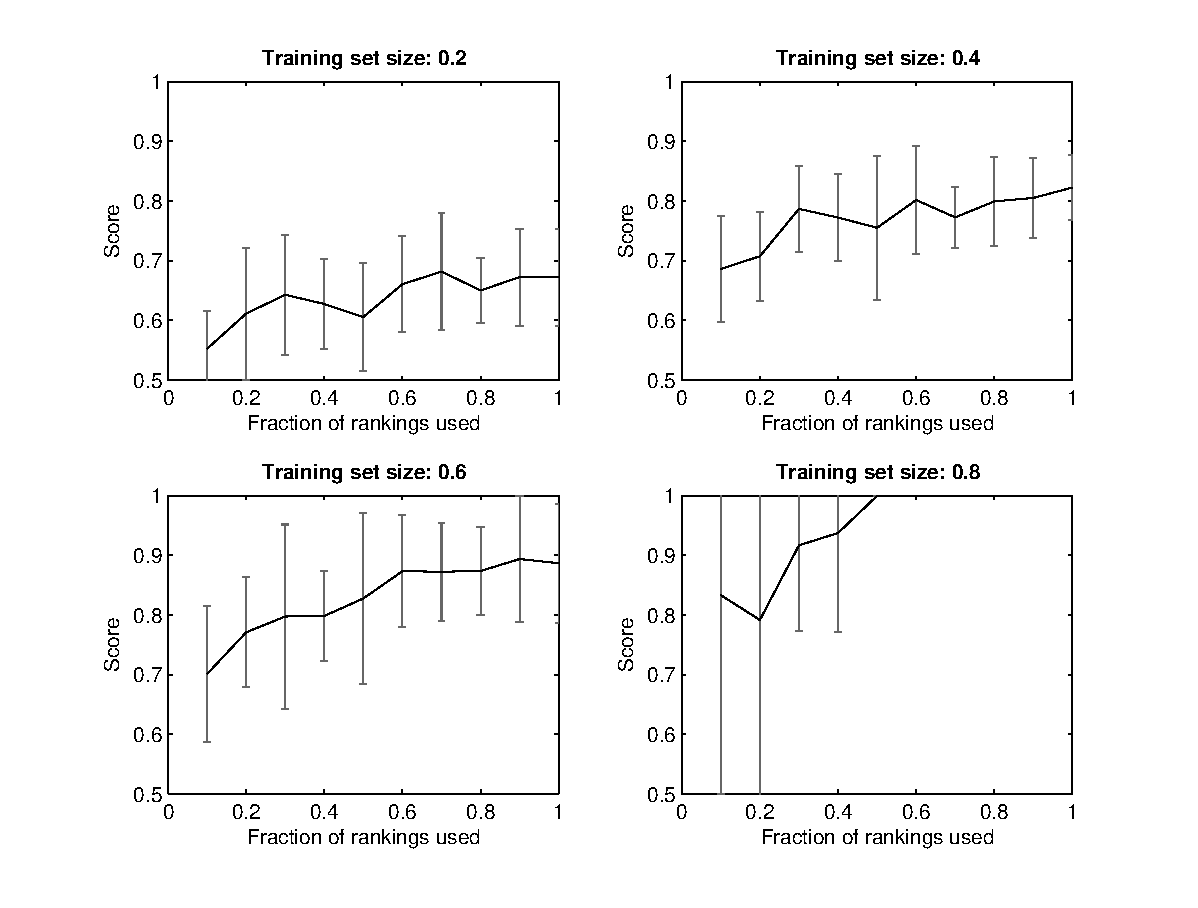
\includegraphics[width=1\linewidth]{rankings}
  \caption{Invloed fractie ongelijkheden}
  \label{fig:fractie}

\end{figure}

Figuur~\ref{fig:fractie} toont aan dat de scores voor grotere leersets en meer beschikbare ongelijkheden toeneemt.
Hierbij worden steeds meer dan 50\% van de paren juist voorspeld en worden redelijk hoge scores behaald zelfs voor kleiner leersets.
Andere experimenten hebben laten zien dat zelfs voor lagere scores de optimalisatie criteria in staat zijn de optimale oplossing te bepalen.
Gelijkaardige scores worden behaald indien het achterliggende model clausules gebruikt die niet door het leersysteem gegenereerd kunnen worden.

\begin{figure}

  \centering
    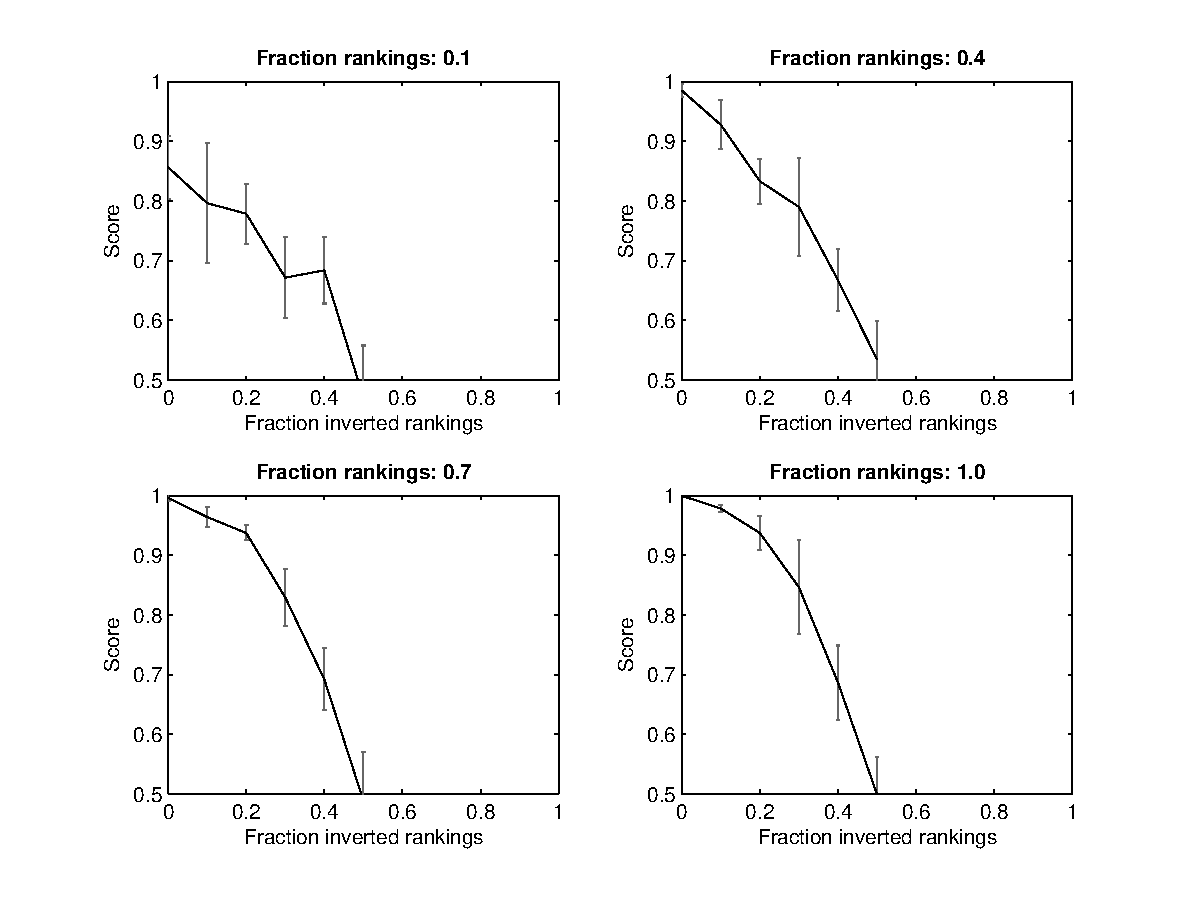
\includegraphics[width=1\linewidth]{noise}
  \caption{Invloed ruis}
  \label{fig:ruis}

\end{figure}

In figuur~\ref{fig:ruis} wordt de invloed van ruis getoond indien alle voorbeelden beschikbaar zijn voor het leren van de zwakke beperkingen.
Het algoritme blijkt bestand te zijn tegen redelijke percentages aan foute rangschikkingen.
Ook bij het gebruik van een leerset met 40\% van de voorbeelden kunnen redelijke scores boven 0.7 behaald worden als 20\% van de rangschikkingen fout zijn.

  \begin{table}
    \caption{Scores voor verschillende limieten ($t$)}
    \begin{tabularx}{\linewidth}{XXXX}
      $t = 1$ & $t = 2$ & $t = 3$ & $t = 4$ \\
      \toprule
     0.823 & 0.740 & 0.788 & 0.735 \\
     ($\pm$ 0.073)&
($\pm$ 0.078)&
($\pm$ 0.074)&
($\pm$ 0.063)
    \end{tabularx}
    \label{tbl:limiet}
  \end{table}

Uiteindelijk toont tabel~\ref{tbl:limiet} dat het verhogen van de limiet voor het vinden van zachte beperkingen de score niet verhoogt.
Het experiment gebruikt een leerset van 40\% en 40\% van de beschikbare ongelijkheden.
Het is wel denkbaar dat voor grotere voorbeelden een hogere limiet wenselijk is.

% An example of a floating figure using the graphicx package.
% Note that \label must occur AFTER (or within) \caption.
% For figures, \caption should occur after the \includegraphics.
% Note that IEEEtran v1.7 and later has special internal code that
% is designed to preserve the operation of \label within \caption
% even when the captionsoff option is in effect. However, because
% of issues like this, it may be the safest practice to put all your
% \label just after \caption rather than within \caption{}.
%
% Reminder: the "draftcls" or "draftclsnofoot", not "draft", class
% option should be used if it is desired that the figures are to be
% displayed while in draft mode.
%
%\begin{figure}[!t]
%\centering
%\includegraphics[width=2.5in]{myfigure}
% where an .eps filename suffix will be assumed under latex, 
% and a .pdf suffix will be assumed for pdflatex; or what has been declared
% via \DeclareGraphicsExtensions.
%\caption{Simulation results for the network.}
%\label{fig_sim}
%\end{figure}

% Note that IEEE typically puts floats only at the top, even when this
% results in a large percentage of a column being occupied by floats.


% An example of a double column floating figure using two subfigures.
% (The subfig.sty package must be loaded for this to work.)
% The subfigure \label commands are set within each subfloat command,
% and the \label for the overall figure must come after \caption.
% \hfil is used as a separator to get equal spacing.
% Watch out that the combined width of all the subfigures on a 
% line do not exceed the text width or a line break will occur.
%
%\begin{figure*}[!t]
%\centering
%\subfloat[Case I]{\includegraphics[width=2.5in]{box}%
%\label{fig_first_case}}
%\hfil
%\subfloat[Case II]{\includegraphics[width=2.5in]{box}%
%\label{fig_second_case}}
%\caption{Simulation results for the network.}
%\label{fig_sim}
%\end{figure*}
%
% Note that often IEEE papers with subfigures do not employ subfigure
% captions (using the optional argument to \subfloat[]), but instead will
% reference/describe all of them (a), (b), etc., within the main caption.
% Be aware that for subfig.sty to generate the (a), (b), etc., subfigure
% labels, the optional argument to \subfloat must be present. If a
% subcaption is not desired, just leave its contents blank,
% e.g., \subfloat[].


% An example of a floating table. Note that, for IEEE style tables, the
% \caption command should come BEFORE the table and, given that table
% captions serve much like titles, are usually capitalized except for words
% such as a, an, and, as, at, but, by, for, in, nor, of, on, or, the, to
% and up, which are usually not capitalized unless they are the first or
% last word of the caption. Table text will default to \footnotesize as
% IEEE normally uses this smaller font for tables.
% The \label must come after \caption as always.
%
%\begin{table}[!t]
%% increase table row spacing, adjust to taste
%\renewcommand{\arraystretch}{1.3}
% if using array.sty, it might be a good idea to tweak the value of
% \extrarowheight as needed to properly center the text within the cells
%\caption{An Example of a Table}
%\label{table_example}
%\centering
%% Some packages, such as MDW tools, offer better commands for making tables
%% than the plain LaTeX2e tabular which is used here.
%\begin{tabular}{|c||c|}
%\hline
%One & Two\\
%\hline
%Three & Four\\
%\hline
%\end{tabular}
%\end{table}


% Note that the IEEE does not put floats in the very first column
% - or typically anywhere on the first page for that matter. Also,
% in-text middle ("here") positioning is typically not used, but it
% is allowed and encouraged for Computer Society conferences (but
% not Computer Society journals). Most IEEE journals/conferences use
% top floats exclusively. 
% Note that, LaTeX2e, unlike IEEE journals/conferences, places
% footnotes above bottom floats. This can be corrected via the
% \fnbelowfloat command of the stfloats package.




\section{Conclusie}
In dit onderzoek werden leersystemen voor beperkingen en optimalisatie criteria ontworpen.
Hiermee konden de vooropgestelde doelstellingen bereikt worden.

Het leersysteem voor beperkingen kon zowel de harde als de zachte beperkingen leren voor alle onderzochte problemen.
Hiermee is het eerste doel van dit onderzoek bereikt.
De problemen konden allemaal opgelost worden in beperkte tijd (minder dan een minuut) en vaak in enkele seconden.
Er werden telkens maar weinig voorbeelden gebruikt om van te leren.
Het systeem stelt minimale eisen aan de gebruiker maar laat toe om expressieve achtergrondkennis te voorzien.
De geleerde beperkingen zijn onafhankelijk van een specifiek domein, dit vergemakkelijkt het opstellen van positieve voorbeelden.

Ook aan het tweede doel van deze thesis, het leren van optimalisatie beperkingen, werd voldaan.
Het leersysteem voor optimalisatie beperkingen kon gewogen beperkingen vinden die toelaten op optimale oplossingen te vinden.
Zelfs bij kleine datasets en ruis op de onderliggende preferenties konden beperkingen gevonden worden waarmee de meeste voorbeelden correct gerangschikt worden.

Naast het faciliteren van het automatische leren van formele representaties kon ook worden uitgewerkt hoe deze representaties kunnen gebruikt worden om (optimale) oplossingen te vinden.
Daarmee is ook een belangrijke stap gezet om interactieve varianten mogelijk maken voor het opstellen van (gewogen) clausules in eerste orde logica. 

\paragraph{Toekomstig werk}
Dit onderzoek biedt veel aanknopingsmogelijkheden.
Het zou interessant zijn om het aantal variabelen en literalen in een clausule dynamisch aan te passen.
Hiertoe kunnen bijvoorbeeld negatieve voorbeelden gebruikt worden.
Door te bepalen wanneer geen negatief voorbeeld meer aanvaard wordt kan het algoritme zelf stoppen.

Het toevoegen van interactiviteit zou de leersystemen kunnen verbeteren, zowel door het genereren van voorbeelden als het vragen om rangschikkingen.
Rangschikkingen kunnen meerdere voorbeelden bevatten, maar gelijkheden worden op dit moment genegeerd.
Nochtans bevatten deze belangrijke informatie, indien een gebruiker deze expliciet opgeeft.

Het feit dat de geleerde clausules onafhankelijk zijn van de specifieke voorbeelden heeft verschillende voordelen.
In sommige gevallen zijn er echter specifieke objecten die eigen zijn aan het probleem zelf.
Het leersysteem zou kunnen uitgebreid worden om globale constanten, die onafhankelijk zijn van specifieke voorbeelden, te ondersteunen. 

% conference papers do not normally have an appendix


% use section* for acknowledgment
\section*{Dankwoord}
De auteur bedankt zijn promotoren Prof. dr. Luc De Raedt en Dr. ir. Anton Dries.
Bovendien is hij dankbaar voor de hulp van Bart Bogaerts, Prof. dr. Jesse Davis, Prof. dr. Marc Denecker en Vladimir Dzyuba.

\end{abstract*}

% A list of figures and tables is optional
%\listoffigures
%\listoftables
% If you only have a few figures and tables you can use the following instead
\listoffiguresandtables

% Now comes the main text
\mainmatter

%!TEX root=Thesis.tex
\chapter{Introduction}
\label{cha:intro}

\begin{figure}

	\caption{From problem to solution}
	\centering
		\includegraphics[width=0.9\textwidth]{ProblemToSolution.pdf}
	\label{fig:problem_to_solution}

\end{figure}

People use computers to solve complex problems, which are hard to solve by hand. Traditionally, this is done by writing programs or algorithms, which are essentially step-by-step instructions that tell the computer how to solve a particular problem. This approach is usually called imperative programming. Alternatively, declarative programming suggests to specify a high level language in which problem can be formulated without specifying how to solve it. Generic programs, called solvers, are used to find solutions to problems formulated in this language. Ideally, a user now just has to focus on formulating his problem. Figure~\ref{fig:problem_to_solution} shows the typical steps to obtain a solution for a problem.

A popular movement within declarative programming is constraint programming. The idea behind constraint programming is that users specify constraints that act upon a set of variables, each of which has a specified domain. It is the task of the constraint solver to assign values from these domains to the different variables such that all the constraints hold. The solver has a lot of freedom in choosing a search strategy and ideally the user does not need to be familiar with the underlying algorithms.

\paragraph{Problem}
Aside from successful applications in research, constraint programming has gained adoption outside of academia and is being used in industrial applications \cite{Simonis:IndustrialApplicationsCP}. Most research, however, is focused on obtaining a solution, giving a representation of the problem. In practice it can however be challenging for non-experts to formulate the constraints to describe their problems. The high learning curve limits the amount of people that can use constraint solvers.

By automating the step of modeling a problem, this thesis attempts to, amongst others, make constraint solving more accessible. In this approach a computer system is used to automatically find constraints using examples of what the user considers valid solutions. The resulting constraints can then be used by an existing constraint solver. [Insert Example !] Constraints can not only be used to describe valid solutions. So called soft constraints express (usually desirable) properties that a solution may or may not fulfill. Solutions that obey desirable soft constraints are considered better than solutions who do not. By assigning weights to soft constraints, an optimal solution can be identified.

The system outlined in this thesis attempts to learn from examples and extract knowledge. It can be used directly by a user trying to model a problem or as part of another program. The system attempts to help users bridge the gap between an unknown problem and obtaining a formal representation. Therefore, it also focuses on being easy to use and make realistic assumptions about what information a user can provide. 

\paragraph{Relevance}
The wide adoption of constraint programming demonstrates its potential to solve complicated problems. It is often used in scheduling and planning applications. However, constraint programming can be used to solve a variety of programming problems \cite{Dymchenki:GoogleCodeJamEclipse}. Improving constraint solvers is an active research domain, which shows there is an interest in using constraint solvers for problem solving.

As stated above there is a substantial effort required to be able to use constraint solvers. This usability problem has already been examined in \cite{Wallace:PrinciplesCP}. The difficulty that many people experience when modeling problems using constraints has already led to several approaches to automate this process. [!! Interest in optimization]

\paragraph{State of the art}
\textbf{\color{red}{[!! Unfinished]}}
Model seeker \cite{Beldiceanu:ModelSeeker} is a system that uses a specialized approach to learn constraints. Other systems like Conacq [Ref Conacq !] and \cite{Lallouet:LearningCP} use algorithms that are based on established machine learning strategies. These systems are examined in chapter \ref{cha:rellit}.

\paragraph{Novelty}
In this thesis, the approach of using established ILP techniques to learn constraints is examined. Research by \cite{Lallouet:LearningCP} and [Ref Quote Andrea ?] has shown that there is potential for exploiting the parallels between ILP and learning constraints. Some of the characteristics of learning constraints are challenging, especially the small set of examples one can typically expect from a user. Therefore, this thesis specifically examines the use of clausal discovery for constraint learning.

Clausal discovery is an ILP algorithm that is adept at identifying structure in small sets of examples. In this thesis the algorithm, which was originally implemented in a system called Claudien, will be revisited. There are some key differences compared to Claudien. The new implementation tries to use information that is easy for a user to provide. Furthermore, some of the key functions in the algorithm are implemented to make use of a generic logical system (ASP solver) instead of Prolog query evaluation. This also enables the use of rich background knowledge, which is passed to the solver. Hereby, this clause learning system can benefit from advances in the field of logical solvers.

So far, there seems to be no other research that has attempted to use this algorithm for constraint learning. [!! Revisit]

Weighted constraints can induce an order over solutions. Given a set of examples, the clause learning system can find soft constraints. The system implemented in this thesis can automatically assign weights to these soft constraints, such that the induced order maximally agrees with user-provided rankings over the given examples. Automatically learning optimization criteria has been done before for propositional formulas [!! Ref Andrea]. In this thesis, this approach is extended to first order logic clauses. Furthermore, instead of using absolute scores over examples, the user preferences are expressed in relative rankings over examples. To our knowledge, these two features have not yet been implemented before.

%!TEX root=Thesis.tex
\chapter{Concepts}
\label{cha:bg}

In this chapter the most important concepts and terms are explained. It is assumed that the reader is familiar with the basics of logic and constraint programming.

\section{Clausal logic}
\label{sec:clausal_logic}
In this thesis constraints are represented as logical clauses. A logical clause consists of a head and a body. In the clause\cen{$H_1, ..., H_n \leftarrow B_1, ..., B_m$,} the atoms $H_1, ..., H_n$ form the head of the clause and $B_1, ..., B_m$ the body. 

Atoms represent facts, that is they are either true or false. Trivially, the logical constants $true$ and $false$ are atoms. Furthermore, an atom can be formed using a predicate symbol and a set of terms, e.g. $friends(Jack, x)$. The predicate symbol is the name of the predicate. Predicates denote relations between terms, which either exist or not. Terms are expressions representing logical objects, either constants (such as $Jack$) or variables (such as $x$). The arity of a predicate is the number of terms it is applied to, e.g. the arity of the previous $friends$ predicate is $2$.

Clauses are in fact a special form of logical implications in which all variables are implicitly universally quantified. The clause mentioned above represents the implication: \cen{$B_1 \land ... \land B_m \Rightarrow H_1 \lor ... \lor H_n$.} Therefore, a clause can also be written as a disjunction of literals: \cen{$\lnot B_1 \lor ... \lor \lnot B_m \lor H_1 \lor ... \lor H_n$.} A literal consists of either an atom or a negation of an atom. Since a clause is a disjunction of literals, adding an atom to the head or the body, will make always make the clause more general. Moreover, a clause can be written as a set: \cen{$\{\lnot B_1, ..., \lnot B_m, H_1, ..., H_n\}$.}

[!! thoery => CNF] Several concepts concerning clauses will be important in the context of this thesis:
\begin{definition}
A clause is functor-free iff all the terms occurring in it are variables.
\end{definition}
Functor-free clauses do not contain constants and are independent of any . Such clauses are generic clauses, in the sense that they are not associated with a specific domain.
\begin{ex}
\label{ex:functor_free}
Consider two domains $\sym{D}_1 = \{MyCat, MyDog\}$ and $\sym{D}_2 = \{John, Suzy\}$ and two clauses \cen{$c_1 = friends(y, x) \leftarrow friends(x, y)$\\
$c_2 = friends(MyDog, x) \leftarrow friends(MyCat, x)$.}
Clause~$c_1$ expresses that friendship is symmetric. It is a functor-free clause and thus independent of the domain. Clause~$c_2$ expresses that all friends of $MyCat$ are also friends of $MyDog$. It is not functor-free and can only be used in the context of $\sym{D}_1$. 
\end{ex}

\begin{definition}
A clause is range-restricted iff there is no variable in the head of the clause which does not also appear in the body of the clause.
\end{definition}

\begin{ex}
Clause~$c_1$ from example~\ref{ex:functor_free} is range-restricted, because the variables occuring in the head ($x$ and~$y$) also occur in the body. On the other hand, the clause \cen{$friends(x, x) \leftarrow true$} is not range-restricted, since the variable~$x$ only occurs in the head.
\end{ex}

\begin{definition}
A clause is connected iff for any two non-empty subsets of terms that occur in the clause, there must be at least one variable which occurs in both subsets.
\end{definition}

\begin{ex}
Consider the clauses \cen{$c_1 = \{friends(x, y), friends(y, z)\}$\\$c_2 = \{friends(x, y), friends(a, b)\}$.} In clause~$c_1$ the two terms in the body of the clause are linked by variable $y$. Therefore, clause~$c_1$ is connected. The two terms occuring in the body of $c_2$, however, do not share a common variable and thus $c_2$ is not connected.
\end{ex}

[!! Explain interpretation?]

\section{Refinement Operator}
A refinement operator is a function $\rho : \sym{L} \mapsto 2^\sym{L}$ that maps an element (clause) in \sym{L} to a set of (child) elements that are also members of \sym{L}. It is used to traverse the search space $2^\sym{L}$. In the context of this thesis, the search space consists of clauses and \sym{L} is the set of atoms that can occur in the clauses. Refinement operators can either specialize or generalize a clause. In the algorithms explored in this research, however, the refinement operator will be used solely for generalization. Therefore, the refinement operator will be assumed to be a generalization operator from now on.

It will be useful to consider the recursive application of a refinement operator $\rho$. Recursively applying $\rho$ means applying $\rho$ to a clause $c$, then to every element in $\rho(c)$ and so on.
\begin{definition}
Given a language \sym{L} and a refinement operator $\rho: \sym{L} \mapsto 2^\sym{L}$, then $\rho^* : \sym{L} \mapsto 2^\sym{L}$ is a function that maps a clause to the total set of clauses that can be obtained by recursively applying $\rho$.
\end{definition}
There are three important properties that a refinement operator can have:
\begin{definition}
A refinement operator $\rho$ is ideal iff every clause in $\rho(c)$ is only minimally more general then $c$.
\end{definition}
Ideality is important in order to fully enumerate a search space. If $\rho$ is ideal then for any pair of clauses $c_s, c_g$ such that $c_g \in \rho(c_s)$, there cannot be a clause $c$ which is more general than $c_s$ and more specific than $c_g$.
\begin{definition}
A refinement operator $\rho$ is complete w.r.t. to a language \sym{L} iff $\sym{L} = \rho^*(\square)$, where $\square$ is the empty clause.
\end{definition}
When considering the recursive application of a refinement operator $\rho$, an element $c_n$ is reachable from $c_1$ iff $c_n \in \rho^*(c_1)$. In that case there is at least one path $(c_1, c_2, ..., c_n)$, where $\forall i > 1: c_i \in \rho(c_{i-1})$. This allows us to define the optimality property:
\begin{definition}
A refinement operator $\rho$ is optimal iff for every element $c_i \in \rho^*(c)$ there is exactly one path from $c$ to $c_i$.
\end{definition}
Optimal refinement operators are desirable because they can be used to search a language space \sym{L} without visiting any element more than once.

\subsection{Object Identity}
The main task of a refinement operator is to calculate the (minimal) generalizations of a clause. Object Identity (OI) is a strategy that is used in order to facilitate this task. Contrary to intuition, in logic two variables $x$ and~$y$ occurring in a clause might denote the same object. Under the OI assumption, however, different variables must denote different objects. This restricts the search space and simplifies the refinement operator. It, however, also limits expressiveness. In practice clauses are expanded with pairwise inequalities between variables. E.g. clause~$c_1$ from example~\ref{ex:functor_free} would be expanded to \cen{$friends(y, x) \leftarrow friends(x, y) \land x \neq y$.}

\section{Bias}
Using a refinement operator, a learning system can traverse the search space of candidate hypothesis. A bias influences the results of the search space, by constraining the search space. Without bias, many search spaces become too large to reasonably explore.

Using clauses to represent constraints is a form of bias, since not all constraints can be expressed using clauses. Several biases have been explored so far. One can restrict the search space to clauses that are range-restricted and\,/\,or connected. Object Identity also forms an important bias on the format of clauses. These all form so called \textit{language} biases. Another form of bias is a \textit{preference} bias. For example, an algorithm can prefer a set of smaller (more specific) clauses over a set of larger (more general) clauses.

Some biases are internal to the learning algorithm. It is, however, also possible to let a user determine a bias. A user can for example limit the maximal number of terms in a clause or provide typing information. Both examples constrain the search space. Such an explicit bias, which can be specified by the user, is called a \textit{declarative} bias.

%!TEX root=Thesis.tex
\chapter{Related Literature}
\label{cha:rellit}

In this chapter, different previous research will be explored.
On the one hand, the state of the art will be described.
On the other hand, research whose contributions this thesis builds on will be explained.

\section{Constraint Learning}
Learning constraints is a difficult problem.
Unlike typical machine learning problems, there is usually little data available from which to learn the constraints.
%While constraint learning is interesting in an automated setting, the goal of some approaches, including this thesis, is also to interact with a human user. This introduces additional difficulties. Human users often lack the skill to 
Different approaches have been taken to tackle this problem.

\subsection{Exisiting approaches}
\paragraph{Learning from queries}
[Info more information needed !] [Ref Quote Note ?]
In order to alleviate the problem of having little data, systems can choose to use queries and user input to guide the search.
[Rewrite "Note mentions" !] Conacq and Quacq [Ref Add refs !] follow this approach. 
Info Does conacq use queries? It uses version space.. ?]

\paragraph{Global constraints and structure}
In constraint programming, one often distinguishes between \textit{local} and \textit{global} constraints.
Local constraints are describe ``simple'' relationships between variables such as $x_1 \neq x_2$.
These constraints can usually not be decomposed.
On the other hand, global constraints describe sets of constraints such as $\mathit{alldifferent}(x_1, x_2, x_3)$.
This global constraint corresponds with a set of local constraints: $x_1 \neq x_2, x_1 \neq x_3, x_2 \neq x_3$.
Besides reducing the number of constraints to model a problem, these global constraints can often be used by a solver to find solutions more efficiently.

Model Seeker \cite{Beldiceanu:ModelSeeker} is an effective approach to constraint learning, which uses global constraints.
It uses generators that structure variables in different ways by arranging them in tensors.
Using a catalog of global constraints, it then tests what global constraints hold in these structures.
This generate-and-test approach has produced good results and works fast.

\paragraph{ILP for constraint Learning}
[Info more text needed !] [Info Introduce CPS etc ?]
One approach that uses parallels between ILP and constraint learning is \cite{Lallouet:LearningCP}.

The approach in this thesis is based on techniques from Inductive Logic Programming (ILP).
Learning systems in this domain often face similar challenges.
ILP attempts to find structure in examples and describe this structure using logical formulas.

\subsection{Clausal Discovery \& Claudien}
\label{sec:claudien}
Claudien, a clausal discovery engine introduced in \cite{DeRaedt:ClausalDiscovery}, attempts to learn a definite clause theory from examples.
Alg. \ref{alg:cd} illustrates how the algorithm works on a high level. 

\begin{algorithm}
	\caption{The clausal discovery algorithm}
	\label{alg:cd}

	\begin{algorithmic}
	\State $\sym{D} \gets Examples$
	\State $Q \gets \{\square\}$
	\State $\sym{T} \gets \{\}$
	\While{$\lnot isempty(Q)$}
		\State $c \gets next(Q)$
		\If{$covers(c, \sym{D})$}
			\If{$\lnot entails(\sym{T}, c)$}
				\State $\sym{T} = \sym{T} \cup c$
			\EndIf
		\Else
			\State $Q \gets Q \cup \rho(c)$
		\EndIf
	\EndWhile
	\State $\sym{T} \gets prune(\sym{T})$
	\State \Return \sym{T}
	\end{algorithmic}
\end{algorithm}

The idea is to start from an empty clause ($\square$).
Clauses are generalized by adding an atom to either the head or the body of the clause in every step, this is the responsibility of the ideal and complete refinement operator $\rho$.
If a clause \obj{c} covers all the examples in \sym{D} and it is not logically entailed by the theory found so far then \obj{c} is added to the result set \sym{T}.
A clause \obj{c} is considered to cover an example \sym{I} iff \sym{I} is a model of \obj{c}: $\sym{I} \models \obj{c}$.
The clause \obj{c} is not refined because any clause $\obj{c_i} \in \rho^*(c)$ is a generalization of \obj{c} and thus logically entailed by \obj{c}.

[Add Bias, (explain why not dlab?) ?]

\subsection{Refinement operator}
The refinement operator plays a central role in clausal discovery, but also in different ILP problems.
General insights about refinement operators have been obtained from \cite{DeRaedt:LRLearning} and are described in chapter \ref{cha:bg}.
In \cite{DeRaedt:CondensedRepresentations} different strategies are discussed that can be used to improve refinement operators, amongst others the canonical form for clauses.

\section{Logical Constraint Solving}
\label{sec:logical_constraint_solving}
There are multiple constraint solvers such as Eclipse and Minizinc [!! Ref Eclipse, Minizinc ?], which use different constraint languages.
Since in this thesis constraints are expressed as logical clauses, it is useful to use a solver which can work directly with first order logic.
This will allow logical background knowledge to be used.

\subsection{IDP}
IDP [!! Ref IDP !] is a knowledge base system which supports an extension of first order logic called FO(.).
This extension includes aggregates, inductive definitions, and other powerful tools for specifying rich background knowledge.
Given a logical theory, IDP is able to perform multiple tasks which are important in this context.
It can check if a model is consistent with the theory, generate a model for a theory as well as expand a partial model.
Because IDP uses SAT solving technology, it is also able to offer the ability to calculate entailment between logical theories.
It is worth noting thath, currently, not all features of FO(.) can be used in entailment.
Performance wise IDP has proven to be amongst the state of the art in multiple answer set competitions [Ref competition !].
Since the system is being actively developed and supported, it is a good choice for a logical solver to be used in this research.

The main difference between a logical solver, like IDP, and traditional constraint solvers, is that the latter class of solvers supports global constraints, programming constructs such as loops and support for (real) numbers.
Global constraints allow constraint solvers to speed up their search and are very compact.
Since the logical constraint generation in this thesis does not focus on global constraints, however, they are not crucial for its implementation.
Additionally, global constraints can usually be emulated using logical background knowledge passed to the solver, if necessary.
Compactness and loops are useful for programmers, but since in this case the constraints are generated automatically these features are less important.
The implicit universal quantification of variables in logical clauses already allows reasoning over domains of variables.
Currently IDP can only reason with natural numbers and contains limited optimization capabilities.
This is its biggest disadvantage.
There is however, a large class of problems that do not require rational numbers.

%!TEX root=Thesis.tex
\chapter{Problem Statement}
\label{cha:problem_statement}

% Concepts
% (Herbrand) Interpretation
% Clause
% Range restricted

%[TODO Write] Given examples we want to learn logical %constraints that describe the data and can be used by a %logical solver to generate models.

%+ We want to model user preferences to be able to find an optimal solution

This thesis attempts to solve mainly two problems: learning constraints from examples and learning optimization criteria from user preferences.
The systems that perform these tasks should be easy to use and take into account what kind of information a user can provide.
Finally, the thesis also outlines how these constraints and optimiztion criteria can be used in practice.

\section{Learning constraints}

The first goal of this thesis is to learn constraints that describe a set of positive examples provided by a user.
Such constraints form a formal representation of a problem.
This formal representation can be used by a constraint solver to generate solutions to the problem.

\label{sec:learning_constraints}

\begin{framed}
	\noindent
	\begin{minipage}{\textwidth}
		\paragraph{Goal 1}
		Given a language of clauses~\sym{L}, a set of examples~\sym{D} and a threshold~$t$, the goal of the constraint learner is to find a complete set $\sym{T} \in 2^\sym{L}$ of maximally specific clauses, that each cover at least $t$ examples in \sym{D}.
	\end{minipage}
\end{framed}

\paragraph{Language}
The language \sym{L} determines what clauses are considered for inclusion in~\sym{T}.
In this thesis, \sym{L} is the language of connected, functor-free and range-restricted clauses (definitions in capter~\ref{cha:bg}) and clauses adhere to object identity.
Object identity specifies that variables with different names cannot denote the same object.
Furthermore, the user explicitly determines the maximal number of variables and atoms per clause, which determines the search space.

\paragraph{Examples}
Formally, examples can be seen as Herbrand interpretations, every example consisting of a set of ground atoms.
A Herbrand interpretation is complete, which means that any facts not included in the interpretation are false.
A clause $c$ is said to cover an interpretation \sym{I} if it is a model of the clause: \cen{$\sym{I} \models \obj{c}$.}
It can often be useful to include domain\,/\,background knowledge.
This knowledge is an input to the learning system and has the form of a logical theory \sym{K}.
If background knowledge is provided, an interpretation \sym{I} is covered, if: \cen{$\sym{I} \models \obj{c} \land \sym{K}$.}
Additionally, users can decide to provide partial interpretations as examples, which are extended to Herbrand interpretations using the background theory.

\paragraph{Threshold}
The threshold $t$ can be used to search for either hard constraints ($t = |\sym{D}|$) or soft constraints, which only have to hold on a subset of \sym{D} ($t < |\sym{D}|$).
This can be useful when constraints might not always hold, for example, when there is noise on the examples.

\paragraph{Learned theory}
A learned theory \sym{T} contains only variables and is independent of the specific examples that were used.
These constraints can, therefore, be used for other problem domains.
For example, constraints learned from a $4 \times 4$ sudoku can, in principle, be used for a $9 \times 9$ sudoku.\footnote{An $n \times n$ sudoku consists of $n$ rows, columns and blocks containing each the numbers $1$ to $n$.}
This an advantage of using first-order logical constraints over propositional constraints.

% \subsection{Evaluating constraints}
% Given the output of the learning phase, this thesis will examine the question: can a theory \sym{T} of learned clauses be used successfully to model constraint problems?

% Systems like IDP have been shown [Ref IDP-solving?] to be able to generate models and extend partial models given a logical theory.
% The success of learning constraints from examples will depend on the quality of the theory generated by the learning system.

\section{Learning optimization criteria}
\label{sec:learning_user_preferences}
\label{sec:learning_optimization_criteria}

The second goal of this thesis is to learn optimization criteria that model the users preferences over a set of examples.
These optimization criteria can then be used to distinguish between better and worse solutions and to identify a optimal solution.

\begin{framed}
	\noindent
	\begin{minipage}{\textwidth}
		\paragraph{Goal 2}
		Given a set of example~\sym{D} and a set of rankings~\sym{P} over these examples, the goal of the clausal optimization process is to find soft constraints~\sym{S} and assign weights to them, such that the order induced by these weighted constraints \sym{W} optimally approximate the rankings in \sym{P}
		% Given a set of soft constraints~\sym{S} and a set of rankings~\sym{P} over an example set~\sym{D}, the goal of the clausal optimization process is to assign weights to every clause in~\sym{S} such that the order induced by the weighted clauses~(\sym{W}) optimally approximate the rankings in \sym{P}.
	\end{minipage}
\end{framed}

\paragraph{Rankings}
The rankings~\sym{P} are partial orderings over examples from~\sym{D}.
Rankings are of the form: \cen{$G_1 > G_2 > ... > G_n$} and every group~$G_i \subset \sym{D}$ is a set of equally ranked examples. Equalities are not used directly by the clausal optimization algorithm, therefore, every ranking corresponds with a set of pairwise (strict) inequalities.

\paragraph{Soft constraints}
The soft constraints are clauses that cover some of the examples in~\sym{D}.

\paragraph{Weighted constraints}
Every weighted constraints consists of a tuple $(w, c) \in \mathbb{R} \times \sym{S}$.
Weights are rational numbers, positive or negative.
The larger the weight of a constraints, the more of a desirable property that constraints forms.
Negatively weighted constraints represent unwanted properties, which should be avoided.

Given a set~\sym{W}, a score $\mathit{score}(\sym{I})$ can be calculated for each interpretation $\sym{I} \in \sym{D}$.
\begin{align*}
	\mathit{score}(\sym{I}) &= \sum\limits_{(w, c)}^\sym{W} w * v(c, \sym{I}) \\
	v(c, \sym{I}) &=
	\begin{cases}
		1,& \text{if } \sym{I} \models c\\
		0,& \text{otherwise}
	\end{cases}
\end{align*}

The $\mathit{score}$ function induces a total ordering over all examples.
Therefore, the weighted constraints \sym{W} can be used as optimization criteria by searching for the interpretation that maximizes the score.

\section{Solving}
Hard constraints in the form of clauses can be used directly by a logical solver to generate solutions.
This is not possible for the optimization criteria that are learned by the clausal optimization process.
To the knowledge of the author, there are no solvers that can use the chosen representation directly.
Therefore, it is a third goal of this thesis to outline how these optimization criteria can be used in practice.

%!TEX root=Thesis.tex
\chapter{Approach}
\label{cha:meth}

In this chapter, the clause learning and clausal discovery systems are outlined.
The clause learning system has the ability to automatically learn clauses from examples.
At the core of the clause learning process is a new version of the clausal discovery system.
The main differences to clausal discovery engine Claudien (see section~\ref{sec:claudien}) are a different bias and a different refinement operator.
Furthermore, the clausal discovery program interacts with a logical system (IDP) to calculate two main functions $\mathit{coverage}$ and \textit{entailment}.

The clausal optimization system uses user-provided rankings and learn-to-rank software (\svm) (see section~\ref{sec:svm}) to produce weighted soft constraints.
These soft constraints are represented as clauses and the clause learning system is used to find these clauses.

Figure~\ref{fig:high_level_structure} provides an overview of the approach implemented in this thesis.

\begin{figure}

	\caption{High level structure}
	\centering
		\includegraphics[width=1\textwidth]{ApproachOverview.pdf}
	\label{fig:high_level_structure}

\end{figure}

Both clause learning and clausal discovery are implemented in Java.
Interaction with the user, the logical system as well as the  software is achieved through files and standard input / output.

Throughout this chapter the map coloring problem will be used as an example for clause learning applications.
In this problem there is a set of countries and every country is assigned a color.
Some countries are neighbors of each other.
The main constraint is that neighboring countries may not have the same color.

\section{Output}
In order to understand the goal of this approach and this thesis, this section will provide more details on the produced outputs.
The aim of the clause learning system is to provide hard or soft constraints that describe valid solutions.
The clausal optimization system produces weighted soft constraints, that can be used as optimization criteria.

\paragraph{Constraints}
For the application at hand, a problem can be viewed as a description of its domain and a set of rules.
The domain consists of all potential solutions to the problems and members of the problem domain will be referred to as instances or models.
If an instance fulfills all the rules, it is considered to be valid or a solution to the problem.
These rules can therefore be seen as \textit{hard} constraints, constraints which an instance must fulfill in order to form a solution to the problem.
Considering, for example, the map coloring problem, then all colored maps are potential solutions.
However, only maps in which countries never have the same color as their neighbors are actual solutions.

In this thesis, constraints are represented as clauses and the clause learning process produces a set (or theory) of clauses.
Using clauses to represent constraints enables the use of learning algorithms from the inductive logic programming and the use of first order logic solvers and background knowledge.

\begin{example}
Given multiple examples of correctly colored maps, the output of the clause learning system would consist of a set of clauses. One of the clauses would express the constraint: \cen{$false \leftarrow color(c_1, color_1) \land neighbor(c_1, c_2) \land color(c_2, color_1)$.}
Because of Object Identity (see chapter~\ref{cha:bg}), variables with different names always denote different object.
\end{example}

Learned clauses can be used to generate new solutions, check if an instance is valid or expand a partial instance into a solution.
The clauses produced by the system are considered hard constraints if they cover all the provided examples.
A user can, however, also provide a custom minimum support value, e.g. $80\%$, then all clauses are returned that cover at least $80\%$ of the provided examples.
This can be used to find constraints that hold most of the time but not always and is also a way to deal with noise on the examples.

\paragraph{Optimization}
Problems potentially have many solutions and not all solutions might be equally good.
Soft constraints are constraints which solutions might fulfill but do not have to.
By using soft constraints, one can discriminate between better and worse solutions.
Every soft constraint has a weight associated with it and every solution can be assigned a score by summing the weights of the soft constraints that it fulfills.

Clausal optimization uses clause learning to find soft constraints in examples.
It then automatically assign weights to them based on the preferences a user expresses over the examples.
For clausal optimization, negative weights are also allowed.
This means that examples that fulfill these negatively weighted constraints actually get scored less than the ones that do not.
Using only positive weights would limit the expressiveness of the weighted clauses as optimization criteria.
One can obtain non-negative weights by negating the clauses that have negative weights.
The resulting logical formula would, however, not be a clause anymore.

The output of the clausal optimization system consists of set of weighted clauses: \cen{$weight_1: clause_1$\\...\\$weight_n: clause_n$.}
For a particular instance \sym{I}, a variable $v_i$ can be introduced for every clause $c_i$.
If $c_i$ is true for \sym{I}, then $v_i$ is $1$, otherwise it is $0$. The score of \sym{I} can then be calculated as:
\begin{equation}
\label{eq:weights_sum}
\sum\limits^n w_i \cdot v_i
\end{equation}

\section{Input}
The input to the clause learning system consists mainly of two parts: definitions and examples.
When learning optimization criteria a third type of information is required: partial rankings over the given examples.
Optionally a user can also provide logical background knowledge.
Background knowledge can be used to impose additional constraints on valid examples, explain how to generate predicates or specify already known facts.

\subsection{Definitions}
The definitions part of the input consists of general information that describes the problem domain and the search space.
This generic information consists mainly of typing information and predicate definitions and is independent of specific examples.

\subsubsection{Typing}
Every object in the problem domain has exactly one type.
Types are declared as:
\begin{shiftedflalign*}
& \textbf{type } Name &
\end{shiftedflalign*}
Using these declared types, objects in the domain can be partitioned into disjoint subsets.
Only using disjoint types limits the capability to correctly model more complicated problems.
Therefore, types are also allowed to have a parent-type.
If an object has type $t$, it belongs to type $t$ and any object that belongs to type $t$ also belongs to the parent-type $p$ of $t$.
Types that have a parent-type are declared as:
\begin{shiftedflalign*}
& \textbf{type } Name \textbf{ > } ParentType &
\end{shiftedflalign*}
Typing information relates directly to the problem domain and is usually easy to provide for the user.
It is valuable to the clause learning algorithm because it restricts the search space.
Because of these two characteristics, it was decided to include typing information as an input.

\begin{example}
	\label{ex:map_color_types}
	The map coloring problem has been described earlier.
	There are two types of objects that are important: countries and colors.
	Therefore, the following type declarations can be formulated:
	\begin{shiftedflalign*}
		& \textbf{type } Country & \\
		& \textbf{type } Color &
	\end{shiftedflalign*}
\end{example}
\subsubsection{Predicate definitions}
Predicates describe relations between objects in a domain.
In the definitions section a user defines the predicates that will be used to describe the relations that exist in the problem domain.
A predicate definition contains information about the name of the predicate, the number of arguments (the arity) and the type of every argument.
A standard predicate is declared as:
\begin{shiftedflalign*}
& \textbf{pred } Name(Type_1, ..., Type_n) &
\end{shiftedflalign*}

There are two variants of predicate definitions.
For a normal predicate like $\mathit{fatherOf}$ the atoms $\mathit{fatherOf}(x, y)$ and $\mathit{fatherOf}(y, x)$ are not equal.
In some circumstances, however, predicates describe symmetric relationships.
Such predicates can be defined as:
\begin{shiftedflalign*}
& \textbf{symm } Name(Type, ..., Type) &
\end{shiftedflalign*}
Symmetric predicates can be used to describe predicates for which the order of the arguments does not matter, e.g. reciprocal friendships or membership of an object in an unordered set.
Since the position of an argument in a symmetric predicate is irrelevant, all arguments must be of the same type.
Defining symmetric predicates allows the user to provide background knowledge he has about a predicate directly to the clause generation algorithm.
Given this information, the system can avoid generating redundant clauses.

The second variant allows the user to specify predicates that are not explicitly provided, but rather are generated according to logical background knowledge provided by the user.
Such calculated predicates are expressed as:
\begin{shiftedflalign*}
& \textbf{calc } Name(Type_1, ..., Type_n) &
\end{shiftedflalign*}

Calculated predicates might be based on the values of other predicates.
In this case a user might want to generate clauses that contain the calculated predicate, but not all of the original predicates.
This is the function of the search directive: 
\begin{shiftedflalign*}
& \textbf{search } Predicate_1\  ...\  Predicate_m &
\end{shiftedflalign*}
Only the specified predicates will be included in the clause learning algorithm.
If no search directive is provided, all defined predicates are included.

\begin{example}
	\label{ex:map_color_predicates}
	In the map coloring problem, there are primarily two relations.
	The \textsc{color} relation specifies the color of a country and the (symmetric) \textsc{neighbor} relation that specifies that two countries are neighbors.
	Considering the types in example~\ref{ex:map_color_types}, the following predicate definitions can be used to express these relations:
	\begin{shiftedflalign*}
		& \textbf{pred } color(Country, Color) & \\
		& \textbf{symm } neighbor(Country, Country) &
	\end{shiftedflalign*}
\end{example}

\subsection{Examples}
While definitions are generic properties of the problem domain, examples describe specific instances or models that the user perceives as valid solutions to his problem.
Every example contains constant declarations that list the objects (constants) that are part of the model as well as their types.
Examples also contain an exhaustive list of the relations that hold on these objects.
\begin{shiftedflalign*}
& \textbf{example }Name\  \{ & \\
& \tabspace \textbf{const } Type\  Object_1\  ...\  Object_k & \\
& \tabspace Predicate(Object_1, ..., Object_n) & \\
& \} &
\end{shiftedflalign*}

\begin{example}
	To illustrate, consider the map coloring problem with the definitions given in example~\ref{ex:map_color_types} and~\ref{ex:map_color_predicates}.
	Consider the countries Belgium, the Netherlands and Luxembourg. Given the fact that Belgium shares a border with the Netherlands and Luxembourg, one example could be:
	\begin{shiftedflalign*}
		& \textbf{example }benelux\  \{ & \\
		& \tabspace \textbf{const } Country\  Belgium\  Luxembourg\  Netherlands & \\
		& \tabspace \textbf{const } Color\  Red\  Blue & \\\\
		& \tabspace neighbor(Belgium, Luxembourg) & \\
		& \tabspace neighbor(Belgium, Netherlands) & \\\\
		& \tabspace color(Belgium, Red) & \\
		& \tabspace color(Luxembourg, Blue) & \\
		& \tabspace color(Netherlands, Blue) & \\
		& \} &
	\end{shiftedflalign*}
	Currently symmetric predicates have to be fully specified, the implementation could, however, easily be changed to automate this.

\end{example}
[!! More details on format?]

\subsection{Logical background knowledge}
In many cases it can be useful to include background knowledge that the user already possesses.
This knowledge can be used to provide additional constraints that a user is aware of, thereby restricting what clauses are considered valid.
A user can also specify facts that he already knows and wants to exclude from the output.
Furthermore, it can be used to automatically calculate predicates.
Consider, for example, two predicates \textsc{crowded(Elevator)} and \textsc{in(Person, Elevator)}.
The examples provided by the user could contain information about which elevator a person is in and the background knowledge could be used to specify that an elevator is crowded if there are more than 8 people in it.

Logical background knowledge is specified in a file.
An important aspect of background knowledge is that it is passed straight to the logical system, as shown in figure~\ref{fig:high_level_structure}.
The format of the background knowledge is thus dependent on the logical system that is being used.

\subsection{Rankings}
Rankings are provided by a user and they express which solutions he prefers.
They are only used for clausal optimization and will be ignored during the clause learning step.
Given examples $e_1, ..., e_x$, rankings are declared as:
\begin{shiftedflalign*}
& \textbf{pref } e_1 = ... = e_i > ... > e_j = ... = e_x &
\end{shiftedflalign*}
This statement expresses that out of examples $1$ to $x$, examples $1$ to $i$ are considered the best and examples $j$ to $x$ the worst examples.
The clausal optimization system will use these rankings to assign weights to soft constraints.
Recall that a score can be calculated for a solution by summing the weights of the soft constraints that cover the solution.
The weights of the constraints are chosen in such a manner that the rankings induced by the score approximate the rankings provided by the user.


An alternative approach would be to use absolute scores for examples.
For a human, however, it is often hard to provide absolute scores over potentially many examples.
Rankings only require the user to consider few examples at a time and express his relative preferences over them.

\section{Clausal Discovery}
\label{sec:clausal_discovery_approach}
As stated previously, clausal discovery forms the core of the clause learning process.
Algorithm~\ref{alg:cd} (section~\ref{sec:claudien}, page~\pageref{alg:cd}) describes the clausal discovery process at a high level.
The behavior of the algorithm is mainly defined by three functions: \textsc{covers(c, \sym{D})}, \textsc{entails(\sym{T}, c)} and \textsc{$\rho$(c)} - the refinement operator.

The algorithm keeps a queue of candidate clauses.
Whenever a clause is selected, it is tested for coverage.
If it succeeds, it is added to the result set, provided it is not entailed by the clauses already in the result set.
If it fails the coverage test, the refinement operator is used to produce generalizations of the clause, which are added to the result set.
Clauses are thus generalized until they pass the coverage test.

\begin{figure}[!htp]

	\caption{Coverage}
	\centering
		\includegraphics[width=0.7\textwidth]{CDCoverage.pdf}
	\label{fig:cd_coverage}

\end{figure}

\paragraph{Coverage} 
Coverage is calculated for each example separately and this calculation is outsourced to the logical system.
If an example violates a clause, the clause is too specific and does not cover the example.
Coverage tests occur frequently and form a significant amount of the total computation time.
These tests can, however, be parallelized to a certain degree, as there is a gap between the moment a clause is added to the queue and the moment it is selected.

\begin{figure}[!htp]

	\caption{Entailment}
	\centering
		\includegraphics[width=0.7\textwidth]{CDEntailment.pdf}
	\label{fig:cd_entailment}

\end{figure}


\paragraph{Entailment}
In order to avoid redundant clauses in the result set, a clause is only added to the result set if it is not logically entailed by the clauses in the result set.
This test is independent the specific examples and is also accomplished by the logical system.
Interaction with the logical system costs time and logical entailment is a hard problem.
Therefore, additional tests are run in the main program to discover some redundancies faster.

\paragraph{Refinement}
If a clause is too specific, it is rejected for not covering enough examples.
It is the task of the refinement operator to generate (minimal) generalizations of a clause, which are added back to the queue.
The refinement operator is thus responsible for exploring the search space.
It dictates what clauses are explored and in which order.
\\\\
In this section the different steps of the clausal discovery implementation will be explored.
The sequence of steps begins at the moment that a new clause is created by the refinement operator.

The algorithm explores the search space in a breadth-first fashion, using a first-in-first-out queue.
Clauses are generalized by the refinement operator by adding one literal to the clause.
Therefore, the clauses are increasing in length over the course of the algorithm.
An important consequence of this process, is that shorter clauses are added to the result set first.
This implies, that the clause is maximally specific.

\subsection{Coverage calculation}
At the moment that a clause is created and to be added to the queue, the computation of the \textsc{covers} function is asynchronously dispatched.
By the time that a clause is selected from the queue, the results from the \textsc{covers} have, in the best case, already been calculated.

\subsection{Subset-test}
When a clause~$c$ is selected from the queue, a subset-test is performed.
The implementation keeps track of the set of clauses \sym{C} that have passed the coverage test, regardless of the result of the entailment test.
As mentioned above, clauses are processed in increasing length.
Assuming a complete refinement operator, any subset of $c$ that forms a valid clause on its own has already been generated.
Any clause has associated with it a set of examples covered by the clause~($c$).
If a subset clause~$c_s$ of~$c$ covers the same examples as~$c$ and $c_s \in \sym{C}$, then $c$ can be safely discarded.

\begin{example}
	Assume~\sym{C} is the set of clauses that have passed the coverage test so far. Consider clauses:
	\cen{$c_1 = \{\lnot p_1(x)\} \notin \sym{C}$\\
	$c_2 = \{\lnot p_2(x)\} \in \sym{C}$\\
	and $c = \{\lnot p_1(x), \lnot p_2(x)\}$.}
	Assume that $c_2$ covers the set of examples $\sym{E}_2$ and $c$ covers examples \sym{E}.
	Since $c_2 \subset c$, it always holds that $\sym{E}_2 \subseteq \sym{E}$.
	If $\sym{E}_2 = \sym{E}$, then the clause~$c$ is redundant because $c_2 \subset c$ is more specific than $c$ and covers the same examples.
	However, if $\sym{E}_2 \subset \sym{E}$, then $c$ covers more examples than~$c_2$ and should also be added to \sym{C}.
\end{example}

\subsection{Coverage-test}
For a clause $c$ to be added to the result set, it must cover a certain number examples.
When looking for hard constraints, all examples must be covered.
Alternatively, a minimum support threshold decides how many examples a clause has to cover.
If the clause covers at least the minimal required amount of examples, it will be submitted to the entailment-test.
If it does not cover enough examples, the refinement operator will be applied to it.

\subsection{Entailment-test}
The entailment tests filters out redundant clauses to obtain a minimal theory.
A clause $c$ is only added to the result set \sym{R} if it is not logically entailed by the clauses that have been added to the result set earlier.
By pruning newer clauses, the algorithm favors short clauses over long clauses.
Clauses are also pruned if they are entailed by the generated or provided background knowledge.
When learning soft constraints, the examples covered by a clause have to be considered.
Only the subset $\sym{R}_c \subset \sym{R}$ of clauses that cover the same examples as $c$ are allowed to prune $c$.
If $c$ is entailed by clauses that cover different examples, then it is still relevant.
\begin{example}
	Consider three examples $e_1, e_2$ and~$e_3$ and clauses:\\

	\begin{tabular}{rl|llll}
		& Clause & Case 1 & Case 2 & Case 3 & Case 4 \\
		\midrule
		$c_1$ & $p_2(x) \leftarrow p_1(x)$ & $e_1$ & $e_1$ & $e_1, e_2$ & $e_1, e_2, e_3$\\
		$c_2$ & $p_3(x) \leftarrow p_2(x)$ & $e_1$ & $e_2$ & $e_1, e_3$ & $e_1$ \\
		$c$ & $p_3(x) \leftarrow p_1(x)$ & $e_1$ & $e_1$ & $e_1$ & $e_1$
	\end{tabular}
	\\\\
	where every case shows the examples covered by each clause.
	Clauses $c_1$ and~$c_2$ logically entail clause~$c$.

	\begin{description}
		\item[Case 1]
			All clauses cover the same examples and $c$ will not be added to the result set because it is redundant.
		\item[Case 2]
			Clause~$c_2$ covers a different example than~$c$.
			Therefore, it cannot be used to prune~$c$ and~$c$.
		\item[Case 3]
			Here, clauses $c_1$ and~$c_2$ both cover a superset of the examples covered by~$c$.
			While clause~$c$ is redundant, it can be used to discriminate $e_1$ from the other examples.
			For example, in the clausal optimization setting, such clauses are useful.
			In order to preserve such clauses, $\sym{R}_c$ does not include soft constraints that cover a superset of the examples that~$c$ covers.
		\item[Case 4]
			This case is related to case~3.
			However, clause~$c_1$ covers all examples.
			Therefore, it is considered to be a hard constraint, like the background knowledge.
			Including these constraints in $\sym{R}_c$ yields a more compact result set at the risk of excluding some clauses if the clauses only covers all examples by chance.
	\end{description}

\end{example}

\subsection{Refinement operator}
In clausal discovery one starts with the empty clause $\square$ and in every step one atom is added to either the head or the body.
Given a clause $c$, the refinement operator $\rho$ returns a set $\rho(\obj{c})$ of child clauses whose length is $length(\obj{c}) + 1$.
What atoms are added to the clause depends on the current clause and the predicates that are used in the search.
The implementation of the refinement operator uses a specific order in which atoms are added to a clause to eliminate duplicate clauses.
Given a maximal amount of variables, a list of possible atoms is generated and every clause is represented as a sorted list of indices referring to elements in the list.
The following section will explain how to generate the list of atoms, such that all possible clauses are at least generated once.

\paragraph{Atom list generation}
The number of arguments of a predicate is referred to as the predicates arity.
A predicate $\obj{p}_3$ of arity 3 takes 3 arguments, e.g. $\obj{p}_3(x, y, x)$.
One can observe that, while the arity of the previous predicate was 3, it only features 2 different variables.
Such a predicate will be considered as having a rank of 2.
Considering Object Identity (see section~\ref{sec:bg_ref_op}), $\obj{p}_3(x, y, x)$ can be viewed as a blueprint for predicates of type $\obj{p}_3$ that feature the first variable on the first and third place and the second -  different - variable on the third place.
This blueprint or predicate prototype represents the function $f^{\obj{p}_3}_{121}(v_1, v_2) = \obj{p}_3(v_1, v_2, v_1)$.

\begin{example}
	The following examples illustrate the use of predicate prototypes:
	\begin{shiftedflalign*}
	f^{\obj{p}_3}_{111}(x) &= \obj{p}_3(x, x, x) \\
	f^{\obj{p}_3}_{121}(x, y) &= \obj{p}_3(x, y, x) \\
	f^{\obj{p}_3}_{123}(x, y, z) &= \obj{p}_3(x, y, z)
	\end{shiftedflalign*}
\end{example}

Given the predicate $\obj{p}_3$ with arity 3, one can construct predicate prototypes of rank 1, rank 2 and rank 3 (see example~\ref{ex:sets_of_prototypes}).
The set $\sym{F}^r_{p_i}$ is then defined as the set of all possible predicate prototypes $f^{p_i}_{x_1, ..., x_n}$ or $f^{p_i}_\mathbf{x}$ of rank $r$.
For every prototype it holds that every number in $[1, r]$ occurs at least once in $\mathbf{x}$ and $max(\mathbf{x}) = r$.

\begin{example}
	\label{ex:sets_of_prototypes}
	For predicate $p_3$, the following sets can be constructed:
	\begin{shiftedflalign*}
		\sym{F}^1_{p_3} &= \{f^{p_3}_{111}\} \\
		\sym{F}^2_{p_3} &= \{f^{p_3}_{112}, f^{p_3}_{121}, f^{p_3}_{211}, f^{p_3}_{122}, f^{p_3}_{212}, f^{p_3}_{221}\} \\
		\sym{F}^3_{p_3} &= \{f^{p_3}_{123}\}
	\end{shiftedflalign*}
\end{example}

In the clausal discovery setting, a user provides a set \sym{P} of predicates that can occur in the generated clauses.
Given a set \sym{P}, the set $\sym{F}^r$ is defined as $\sym{F}^r = \bigcup \{\sym{F}^r_{p_i} | p_i \in \sym{P}\}$.
Such a set contains all predicate prototypes of rank $r$.
The reader may recall that these prototypes are actually functions that map variables to a predicate.
Therefore, $\sym{F}^r$ can also be used as a function that takes $r$ variables and maps them to the set of predicates, obtained by applying every function in $\sym{F}^r$ to those $r$ variables.

\begin{example}
	Consider $\sym{P} = \{p_1, p_2\}$:
	\begin{shiftedflalign*}
		\sym{F}^1 &= \{f^{p_1}_{1}, f^{p_2}_{11}\} \\
		\sym{F}^1(x) &= \{p_1(x), p_2(x, x)\}
	\end{shiftedflalign*}
\end{example}

Finally, suppose the maximal number of variables is 3 and the maximal arity of the given predicates is 2, then the atom list for this problem is:
\begin{align*}
\sym{L} = \sym{F}^1(v_1) \cup \sym{F}^2(v_1, v_2) \cup \sym{F}^2(v_1, v_3) \cup \sym{F}^1(v_2) \cup \sym{F}^2(v_2, v_3) \cup \sym{F}^1(v_3)
\end{align*}
Any clause with 3 variables can be represented as an ordered sequence of atoms drawn from this list.
The list is sorted by variables, where $v_1 < v_2 < v_3$, and then predicates.
For example $\sym{F}^3(v_1, v_2, v_3)$ would occur before $\sym{F}^2(v_1, v_3)$.

\begin{example}
	\label{ex:ref_op_list}
	Consider, again, $\sym{P} = \{p_1, p_2\}$ and 2 variables, then:
	\begin{shiftedflalign*}
		\sym{L} &= \sym{F}^1(v_1) \cup \sym{F}^2(v_1, v_2) \cup \sym{F}^1(v_2) \\
		&= \{p_1(v_1), p_2(v_1, v_1), p_2(v_1, v_2), p_2(v_2, v_1), p_1(v_2), p_2(v_2, v_2)\}
	\end{shiftedflalign*}

	The clause $c = p_2(v_1, v_1) \leftarrow p_1(v_1) \land p_2(v_1, v_2)$ can be written as $\sym{L}(2) \leftarrow \sym{L}(1) \land \sym{L}(3)$ or $\{\lnot \sym{L}(1), \lnot \sym{L}(3), \sym{L}(2)\}$.
\end{example}

\paragraph{Building clauses}
The refinement operator uses the atom list to generalize clauses by adding atoms which occurs later in the atom list.
Clauses are build in two stages.
In the first stage, atoms are added to the body.
In the second stage, atoms are added to the head.
Before the second stage, the atom list is reset.
Atoms that have been added in the first stage cannot be added in the second stage (this would result in a redundant clause that is always true).

\begin{example}
	The clause shown in example~\ref{ex:ref_op_list} would be build as follows:
	\begin{shiftedflalign*}
		\textit{Stage 1 }  & \{\lnot \sym{L}(1)\} \\
		& \{\lnot \sym{L}(1), \lnot \sym{L}(3)\} \\
		\textit{Stage 2 }  & \{\lnot \sym{L}(1), \lnot \sym{L}(3), \sym{L}(2)\} = c
	\end{shiftedflalign*}

	The refinement operator would then generate the following clauses:
	\begin{shiftedflalign*}
		\rho(c) = \{
			&\{\lnot \sym{L}(1), \lnot \sym{L}(3), \sym{L}(2), \sym{L}(4)\}
				%(p_2(v_2, v_1) \lor p_2(v_1, v_1) \leftarrow p_1(v_1) \land p_2(v_1, v_2))
			\\
			&\{\lnot \sym{L}(1), \lnot \sym{L}(3), \sym{L}(2), \sym{L}(5)\}
				%(p_1(v_2) \lor p_2(v_1, v_1) \leftarrow p_1(v_1) \land p_2(v_1, v_2))
			\\
			&\{\lnot \sym{L}(1), \lnot \sym{L}(3), \sym{L}(2), \sym{L}(6)\}\}
				%(p_2(v_2, v_2) \lor p_2(v_1, v_1) \leftarrow p_1(v_1) \land p_2(v_1, v_2))
	\end{shiftedflalign*}
\end{example}

\paragraph{Syntactic restrictions}
Different restrictions limits what clauses are generated.
One such restriction is typing information, which is used statically and dynamically.
When the atom list is generated, atoms that are inconsistent with respect to the typing information of the predicates are removed from the list.
During the algorithm atoms that are inconsistent with the types that have been assigned to variables are not added.

\begin{example}
	Typing restrictions are illustrated on some examples using a type $T$ and two disjoint subtypes $S_1$ and $S_2$ of $T$.

	\begin{table}[!htp]
		\begin{tabularx}{\textwidth}{llX}
				\textbf{Type definition} & \textbf{Atom} & \textbf{Prune?} \\
				\toprule
				$p_2(S_1, S_2)$ & $p_2(v_1, v_1)$ & Statically \\
				$p_2(T, S_1)$ & $p_2(v_1, v_1)$ & Dynamically if $\mathit{type}(v_1) \neq S_1$ \\
				$p_1(T)$ & $p_1(v_1)$ & No (if there are no other types) 
		\end{tabularx}
	\end{table}

\end{example}

Clauses must also be connected and range restricted, which is checked at runtime.
To check if an atom~$a$ can be added to a clause~$c$, consider $V_a$, the set of variables occurring in~$a$ and $V_c$, the variables occurring in~$c$.
If $min(V_a) > max(V_c)$, then the atom is not added because the clause would not be connected.
Additionally, if more than one new variable is introduced in a new atom, they must be introduced in increasing order to avoid the generation of duplicate clauses.
If the clause is in stage 2 and $max(V_a) > max(V_c)$, then the atom is not added because the clause would not be range restricted.

This order of the atom list is important, because it assures that clauses are generated in a connected way by placing connecting atoms first.
For example, clauses containing only $v_2$ are generated after clauses that contain $v_1$ and~$v_2$.
Therefore, dropping the $k$ last literals always results in a valid, connected clause.

\paragraph{Representative clause}
Often a clause is not unique and there are multiple ways to formulate it.
Even though the use of the atom list removes most duplicates, there are still some clauses that are reformulations of other clauses.

\begin{example}
	Consider the graph coloring predicates $\mathit{neighbor}$ and $\mathit{color}$ and clauses:
	\begin{shiftedflalign*}
		c_1 &= \{\lnot \mathit{color}(v_1, v_2), \lnot \mathit{neighbor}(v_1, v_3)\} \\
		c_2 &= \{\lnot \mathit{neighbor}(v_1, v_2), \lnot \mathit{color}(v_1, v_3)\}
	\end{shiftedflalign*}
	Then clause~$c_2$ is just a reformulation of the clause~$c_1$.
\end{example}

\begin{example}
	A more complex example are the clauses:
	\begin{shiftedflalign*}
		c_3 &= \{\lnot \mathit{color}(v_1, v_2), \lnot \mathit{neighbor}(v_1, v_3), \lnot \mathit{color}(v_4, v_2)\} \\
		c_4 &= \{\lnot \mathit{color}(v_1, v_2), \lnot \mathit{color}(v_3, v_2), \lnot \mathit{neighbor}(v_3, v_4)\}
	\end{shiftedflalign*}
	These clauses again formulate the same constraint.
\end{example}

These duplicates are harder to detect, especially the second example.
To solve the problem of detecting these duplicates, this thesis suggests a procedure which will be referred to as ``representative test''.

The first step for detecting these duplicates is to define an order that specifies that, for example, clause~$c_3$ is ``smaller'' than clause~$c_4$.
This order can be provided by the atom list and looking at the positions of the smallest atom that does not occur in the other clause.

Using this order the representative clause can be defined as the smallest clause of all equivalent clauses.
If the current clause is the representative clause it is generated, otherwise is not.
The representative clause for a clause~$c$ is found by shuffling the literals in the clause.
If a shuffled clause can be built using the refinement operator that is smaller than the clause~$c$, $c$ can be discarded.

\begin{example}
	This example illustrates how the representative test dismisses clause~$c_4$.
	\begin{shiftedflalign*}
		c_4 = &\{\lnot \mathit{color}(v_1, v_2), \lnot \mathit{color}(v_3, v_2), \lnot \mathit{neighbor}(v_3, v_4)\} \\
		\mathit{shuffle} :\  &\{\lnot \mathit{color}(v_3, v_2), \lnot \mathit{neighbor}(v_3, v_4), \lnot \mathit{color}(v_1, v_2)\} \\
		\mathit{reorder\  variables} :\  &\{\lnot \mathit{color}(v_1, v_2), \lnot \mathit{neighbor}(v_1, v_3), \lnot \mathit{color}(v_4, v_2)\} = c_3 < c_4\\
	\end{shiftedflalign*}
\end{example}

There is only one representative clause for every clause and if a clause is not representative is it discarded.

\begin{proof}
	A representative clause must contain the same number of variables and the same predicates as the original clause.
	Since variables are introduced in a strict order, only the placement of the predicates can vary.
	There is exactly one minimal placement that results in a valid clause, as there must be at least one different literal.

	By generating permutations of literals in a clause, all possible placements of predicates are considered.
	Therefore, the representative clause must also be generated.
\end{proof}

% \paragraph{Optimality}
% In chapter~\ref{cha:bg} the notions of completeness and optimality for refinement operators are introduced.
% A refinement operator is complete if every clause is visited at least once and it is optimal if every clause is visited but once.

% The refinement operator suggested in this thesis is considered to be optimal, with respect to Object Identity and syntactic restrictions.

% \emph{(Completeness)}
% 	Any clause can be written as a set of literals from the atom list and therefore, it can be built incrementally.
% 	As shown previously, any clause can also be rewritten into a representative clause.
% 	The order of the atom list is chosen such that connecting literals are generated first.
% 	As a result, if the $k$ last literals of a clause $c$ are dropped, the resulting clause $c_k$ is also connected.
% 	A property of a representative clause is, that the clause 


% 	Leaving out the last $k$ literals $E_k$
% 	If the clause $r - e$ is generated, than $r$ will also be generated.
% 	But, since $r$ was representative, so must $r - e$.
% 	Otherwise a permutation of $r$ would be smaller than $r$ which is not possible since $r$ is representative.


% removing the last literal results in a valid clause, and if that clause is generated, then so will 


% Clauses that are 

\paragraph{Symmetric predicates}
For symmetric predicates the order of terms is irrelevant.
Internally, these predicates are always reduced to a unique form by ordering the variables that  occur in it.
Atoms that contains symmetric predicates with out-of-order variables can be deleted from the atom list.

\subsection{Pruning}
After the algorithm is finished, the resulting theory is pruned, because newer clauses could entail older clauses.
The procedure used for pruning is the same as for entailment.
For each clause an entailment test is run to see if the clause is entailed by the rest of the theory.
The resulting theory is more compact, without loosing expressiveness.

\section{Logical system}
\label{sec:logical_system}
One of the key features of the clause learning system implemented for this thesis, is the use of a logical system to compute two core functions: coverage and entailment.
The clausal discovery implementation makes use of a generic  interface - the LogicExecutor - to interact with a logical system.
An implementation of this interface provides the interaction with a specific system.

Currently, the clause learning implementation uses the IDP knowledge base system, which was described briefly in section~\ref{sec:logical_constraint_solving}.
IDP uses $FO(\cdotp)$, an extension of first order logic, which supports types, aggregates, inductive definitions and more.
Since the entailment functionality does not currently support all of these features, including these features in the background theory will require either providing a more limited theory for entailment than for coverage or suppressing the entailment test.

IDP uses three elements to describe problems and constraints.
The first element is a vocabulary which contains type and predicate definitions.
Secondly, theories consisting of $FO(\cdotp)$ statements are used to express constraints.
The third element are structures, which represent partial or total instances or models.

\begin{figure}

	\caption{Conversion process}
	\centering
		\includegraphics[width=0.6\textwidth]{Coverage.pdf}
	\label{fig:conversion_to_logic}

\end{figure}

Figure~\ref{fig:conversion_to_logic} shows how to convert the different available information into the elements that IDP works with.
The vocabulary is generated from typing information and predicate definitions, while examples are converted to structures.
User provided background knowledge is already given in the form of a theory $\sym{B}_U$ and generated background knowledge - for symmetric predicates - is converted into a theory $\sym{B}_G$.
In IDP these two theories are then merged into a background theory \sym{B}.
Given the knowledge base, different types of inference can be run in IDP by defining procedures in the Lua scripting language.

\subsection{Coverage}
\textsc{covers(c, \sym{D})} calculates whether a clause $c$ covers the data \sym{D}.
In order to compute this function, a knowledge base and a procedure have to be synthesized.
Vocabulary, structures and background theory are generated as described above and the clause $c$ is converted to a logical theory $\sym{T}_c$.
For every example $e_i$ a structure $\sym{S}_i$ is generated.
The procedure in IDP attempts to expand each structure $\sym{S}_i$ with respect to $\sym{B} \cup \sym{T}_c$.
If such a model exists, $c$ is considered to cover $e_i$.
In practice the coverage for every example is calculated and the results are sent back to the clause learning algorithm.

\subsection{Entailment}
\textsc{entails(\sym{T}, c)} computes whether a theory \sym{T} entails the clause $c$.
The theory \sym{T} represents the theory formed by all clauses that have been found to cover the data so far.
It also contains the available background knowledge.d
IDP offers the capability to compute entailment between two theories.
This logical entailment is independent of any structures and uses a built-in SAT solver.
Aside from generating the vocabulary and background theories as usual, the theories $\sym{T}_R$ and $\sym{T}_c$ are calculated.
These represent the theory of clauses in the result set and of the given clause, respectively.
\sym{T} is then formed as $\sym{T} = \sym{B} \cup \sym{T}_R$ and using IDP it is calculated if \sym{T} entails $\sym{T}_c$.
The (boolean) result is returned to the clause learning system.
Using logical entailment identifies redundant clauses.
Not only does it identify clauses that are reformulations of each other, it also removes clauses which are a combination of other clauses.

\section{Clausal Optimization}
\label{sec:clausal_opt_approach}
Clausal optimization needs two inputs: a set of (learned) clauses that each cover some, but not all of the provided examples as well as a set of rankings provided by the user.
Every ranking concerns a subset of the available examples.
The goal of clausal optimization is to discriminate between examples, based on soft constraints that hold on the examples, and approximate the given rankings optimally.

\paragraph{Soft constraints}
The soft constraints which are to be used as optimization criteria are learned using clause learning with a minimum threshold of 1 example.
Soft constraints with a low support can be interesting, for example, to distinguish between good (bad) solutions and the best (worst) solutions.
Since such constraints might also be due to over-fitting, the threshold could be increased if many examples are available.
Hard constraints are not used for ranking as they hold for all examples.

\paragraph{Learn to rank}
Examples are characterized by the soft constraints (clauses) which cover them.
Therefore, every example can be translated into a vector of boolean features.
Each feature $f_i$ corresponds with one of the clauses and is \emph{1} if the clause covers the example and \emph{0} otherwise.
Now existing machine learning software can be used to learn a linear function $\sum_i w_i \cdot f_i$ over these features, based on the given rankings.
For an unseen example, the feature vector is computed by calculating what clauses cover the new example.
That linear function can then be used to calculate a score for that example.

\begin{example}
	Consider examples~$e_1, e_2, e_3$, rankings $e_1 > e_2, e_2 > e_3$ and clauses $c_1, c_2, c_3$.
	If the clauses cover examples according to table~\ref{tbl:cover_examples}, then the function $(1 \cdot c_1) + (0\cdot c_2) + (-2\cdot c_3)$ perfectly models the given rankings.
	An example $e_4$ that is covered by~$c_1$ and~$c_2$, is then assigned a score of $1$.
	This score has no value in the absolute sense, it can only be used to compare it to other examples ranked by the same function.

	\begin{table}[!htp]
	\label{tbl:cover_examples}
	\begin{tabularx}{\textwidth}{c|ccc|X}
		\textbf{Clauses}	&$c_1$  	& $c_2$ 	& $c_3$ 	& \textbf{Feature vector}\\
		\toprule
		$e_1$ 				& Covers 	&  			&  			& 1, 0, 0\\
		$e_2$ 				& 			& Covers	&  			& 0, 1, 0\\
		$e_3$ 				& Covers 	& Covers 	& Covers 	& 1, 1, 1\\
	\end{tabularx}
	\caption{Clause coverage}
	\end{table}

\end{example}

In this thesis \svm{} was chosen to accomplish this task.
[!! "Why \svm{}?"]

\paragraph{Cost}
Weights are chosen optimally with respect to a cost parameter $c$, which determines the trade-off between disagreeing with a user provided ranking and a simpler model.
Assigning a low cost to disagreeing with the training rankings establishes a bias towards simpler models which can avoid over-fitting the training.
A high cost should be assigned, however, when one is interested in a model that is more accurate with respect to the given examples and rankings.

\section{Solving}
Using the clause learning and clausal optimization system enables a user to find formal representation of the constraints that describe the problem and user's preferences.
Clauses can be used in IDP to generate or check solutions to a problem by providing the learned constraints, defining a partial structure and performing model expansion on it.
It may be necessary to supply some additional information, such as that every country needs to be assigned a color.

\paragraph{MAX-SAT}
Weighted clauses can be obtained using the clausal optimization process.
Soft constraints found by the clause learning process can also be transformed into weighted clauses by using their frequency as a weight.
The problem of finding optimal solutions for these weighted clauses can be seen as a first order generalization of weighted MAX-SAT problem (see section~\ref{sec:max_sat}).

Solvers for weighted MAX-SAT attempt to optimize a formula consisting of a conjunction of positively weighted propositional clauses, by assigning values to the variables occurring in the formula.
In this thesis, first order logic clauses are used and the weights assigned to them can be positive or negative.
The optimization task is then very similar to the MAX-SAT setting:
Assign values to the variables such that the sum of the weights of the clauses that are satisfied is maximized.

\paragraph{Solving}
This optimization task can be solved directly in IDP, using inductive definitions, aggregates and minimization.
The only limitation is that the weights must be integer values.
Therefore, the weights of the clauses are divided by the smallest absolute weight, multiplied by a constant and rounded to the closest integer if necessary.
Removing this restriction for IDP is currently being researched and future releases might be able to deal with rational numbers directly.

In order to model the optimization problem in IDP, every clause $c_i$ with variables $v_1, ..., v_n$ is represented by a number $i$. For every clause a predicate $t(i)$ is added to capture the truth value of the clause.
A function $\mathit{cost}(i)$ specifies the cost of not satisfying the clause, which is equal to the integer weight of the clause.
\begin{shiftedflalign*}
	t(i) &\Leftrightarrow \forall v_1, ..., v_n : c_i. \\
	cost(i) &= w_1.
\end{shiftedflalign*}

Using $t$ and $\mathit{cost}$, a function $\mathit{actual}(i)$ is then defined in IDP as 0 if $t(i)$ and $\mathit{cost}(i)$ if $\lnot t(i)$.
This function is used in the term $\sum_i actual(i)$ to be minimized, which will allow IDP to search for an optimal solution.
The term can be expressed in IDP using the sum aggregate:
\begin{shiftedflalign*}
	sum\{i, cost : actual(i) = cost : cost\}
\end{shiftedflalign*}

The IDP code for a set of learned weighted clauses can easily be generated automatically.
An example is provided in appendix~\ref{app:co_idp}.

%!TEX root=Thesis.tex
\chapter{Evaluation}
\label{cha:evaluation}

% \begin{table}[!htp]
% 	\begin{tabularx}{\textwidth}{r|llllllX}
% 	    \toprule
% 	    Circles & 7 & 8 & 9 & 10 & 11 & 12 & 13  \\
% 	    \midrule
% 	     30 seconds & 0.976 & 0.962 & 0.948 & 0.905 & 0.891 & 0.859 & 0.852\\
% 		 60 seconds & 0.976 & 0.977 & 0.944 & 0.957 & 0.908 & 0.902 & 0.915\\
% 		 90 seconds & 0.978 & 0.951 & 0.971 & 0.952 & 0.886 & 0.937 & 0.901\\
% 		120 seconds & 0.978 & 0.953 & 0.968 & 0.928 & 0.916 & 0.913 & 0.898\\
% 	    \bottomrule
% 	\end{tabularx}
% 	\label{tbl:lin-best}
% 	\caption{Best relative scores of linear method}
% \end{table}

Several experiments have been run in order to assess how well the implementation accomplishes the clause learning and clausal optimization tasks.
Moreover, the influence of different factors internal and external to the algorithm is evaluated.
The clause learning and clausal optimization workflows will be examined separately, in that order.

\section{Learning}

This section attempts to evaluate how well the clause learning system accomplishes the first goal of this thesis.
There are different aspects to be considered.
Firstly, the accuracy of the learned clauses will be examined, as well as the influence of several parameters on the accuracy.
This gives a measure of how well a learned theory approximates the underlying model.
Secondly, it will be evaluated how efficiently this task is accomplished.
Since clausal discovery can take a long time to find a theory on larger examples, it will be important to understand the influence of several factors on the running speed.
In the last part, the differences between learned clauses and constraints given by a user will be examined.

\subsection{Setup}
There are two key problems that are used to evaluate different questions.
Their standard setup will be described in this section.
Different experiments can vary on the specific examples and parameters that are used and it will be mentioned when this is the case.

\paragraph{Map coloring}
The map coloring problem has already been used as a running example in the previous section.
It also serves as a good, albeit small, example for clause learning in practice.
The standard setting uses two examples, each with three countries.
The first example (figure~\ref{fig:setup_mapcolor_benelux}) features two colors, while the second example (figure~\ref{fig:setup_mapcolor_benede}) needs three colors as all countries are connected.

\begin{figure}
\centering
\begin{minipage}{.5\textwidth}
  \centering
  \includegraphics[height=3.5cm]{MapColoringBenelux.pdf}
  \caption{Map coloring example 1}
  \label{fig:setup_mapcolor_benelux}
\end{minipage}%
\begin{minipage}{.5\textwidth}
  \centering
  \includegraphics[height=3.5cm]{MapColoringBenede.pdf}
  \caption{Map coloring example 2}
  \label{fig:setup_mapcolor_benede}
\end{minipage}
\end{figure}

Map coloring uses types $\mathit{Country}$ and $\mathit{Color}$.
It uses two predicates $\mathit{color/2}$ and $\mathit{neighbor/2}$, the neighbor predicate is symmetric.
Unless mentioned otherwise, the standard parameters for map coloring are $3$ variables and~$3$ terms per clause.

\paragraph{Sudoku}
Sudoku is a slightly more difficult problem.
An $n \times n$ sudoku contains $n$ rows, $n$ columns and $n$ blocks, each of which contains the numbers $1$ to $n$ exactly once.
Every cell is represented by an object of type $\mathit{Cell}$.
The other types describe attributes of cells: $\mathit{Row}$, $\mathit{Colum}$, $\mathit{Block}$ and a numeric type $\mathit{Value}$.
Each of those attributes is related to a cell through the predicates $\mathit{row/2}$, $\mathit{col/2}$, $\mathit{block/2}$ and $\mathit{value/2}$ respectively.
In the standard setting one $4 \times 4$ example (figure~\ref{fig:setup_sudoku}) is provided.

\begin{figure}[!htp]
	\centering
	\begin{tabular}{|cc|cc|}
		\hline
		1 & 3 & 2 & 4 \\
		4 & 2 & 3 & 1 \\ \hline
		2 & 1 & 4 & 3 \\
		3 & 4 & 1 & 2 \\ \hline
	\end{tabular}
	\label{fig:setup_sudoku}
	\caption{$4 \times 4$ sudoku example}
\end{figure}

Clause learning on the sudoku is usually done with $4$ variables and~$4$ terms per clause.
In the example, the row, column, block and value are explicitly given for each cell.
The use of specific, disjoint types instead of one common (numeric) type for rows, columns and blocks makes the clause learning process more efficient.
It prevents the use of the same variable for, for example, a row and a column.

\paragraph{Elevator}

\paragraph{Co-housing}
The co-housing problem is a somewhat more complex problem.
Two friends (persons) are looking at different situations (areas) to live and work in.
\\\\
\begin{minipage}{0.5\textwidth}
	\begin{verbatim*}
		type Area
		type Person
		type Cost > nat

		calc cheap(Cost)
	\end{verbatim*}
\end{minipage}
\begin{minipage}{0.5\textwidth}
	\begin{verbatim*}
		pred live(Person, Area)
		pred work(Person, Area)
		pred car(Person)

		pred cost(Area, Cost)
	\end{verbatim*}
\end{minipage}

Background knowledge is used to calculate what is considered as cheap. It also limits the amount of people to $2$ and expresses that every area has only one cost. There are $5$~examples that each adhere to $4$~constraints:

\begin{enumerate}
	\item If the two persons do not live in the same area, they work in the same area.
	\item If a person does not work and live in the same area, that person needs a car.
	\item A person who lives in a cheap area has a car
	\item If the two persons live together, they live in an expensive area.
\end{enumerate}

\subsection{Accuracy}

\# Q : Does the learned theory express the model
% - P Observation (Additional [-> IDP?] | Essential | Damaging)
% - N Test examples

\# Q : Influence parameters
% - C Influence number terms / variables
% - N Dependent of size / number of examples
% - C Influence range restriction

\subsection{Speed}

Unless explicitly stated, all problems are run $8$ consecutive times in order to eliminate external influences.
The experiments are run on the same machine\footnote{Mac OSX, 2.3 GHz Intel Core i7 with 4 cores and hyper threading, 16GB RAM}.

\begin{question}
	How fast is the clause learning system?
\end{question}

\begin{experiment}
	In order to gain an overview over the running times and provide a benchmark for tests on various influences, the standard examples are each run using the standard clause learning process.
	
	\begin{table}[!htp]
		\begin{tabularx}{\textwidth}{XXX}
			\textbf{Name}	& \textbf{Mean (s)}	& \textbf{StdDev (s)} \\
			\toprule
			Map coloring 	& 1.581				& 0.117 \\
			Sudoku 			& 4.787				& 0.062 \\
			Elevator 		& 3.182 			& 0.073 \\
			Co-housing 		& 25.903			& 0.446
		\end{tabularx}
		\label{tbl:exp_speed_standard}
		\caption{Running times for standard examples}
	\end{table}

\end{experiment}

% - N Compared with others?

\paragraph{Discussion}
"Discuss"

\begin{question}
	What is the influence of the various parameters and input data?
\end{question}

% - C Influence number terms / variables
% - N Influence number examples
% - N Influence arity

\begin{question}
	How do the syntactic restrictions influence the running time?
\end{question}

\begin{experiment}[\textsc{Range restriction}]
	The clause learning algorithm normally only explores range restricted clauses.
	While this measure positively influences the efficiency of the algorithm, it trades off expressiveness.
	In this experiment the standard problems are run, while allowing lifting the constraint that clauses must be range restricted.

	\begin{table}[!htp]
		\begin{tabularx}{\textwidth}{XXX}
			\textbf{Name}	& \textbf{Mean (s)}	& \textbf{StdDev (s)} \\
			\toprule
			Map coloring 	& 4.629				& 0.199 \\
			Sudoku 			& 16.118			& 0.154 \\
			Elevator 		& 40.453 			& 0.319 \\
			Co-housing 		& 207.768			& 0.330
		\end{tabularx}
		\label{tbl:exp_speed_standard}
		\caption{Running times for standard examples without range restriction}
	\end{table}

\end{experiment}

\begin{experiment}[\textsc{Connected clauses}]
	"Write"

	\begin{table}[!htp]
		\begin{tabularx}{\textwidth}{XXX}
			\textbf{Name}	& \textbf{Mean (s)}	& \textbf{StdDev (s)} \\
			\toprule
			Map coloring 	& 1.589				& 0.110 \\
			Sudoku 			& 7.068				& 0.150 \\
			Elevator 		& 6.157 			& 0.114 \\
			Co-housing 		& 103.633			& 0.131
		\end{tabularx}
		\label{tbl:exp_speed_standard}
		\caption{Running times for standard examples without range restriction}
	\end{table}

\end{experiment}

\paragraph{Discussion}
"Discuss"

\begin{question}
	What is the influence of the efficiency measures on the running time?
\end{question}

There are mainly two measures incorporated in the clause learning algorithm that aim to reduce the running time.
Contrary to syntactic restrictions these do, in principle, not affect the outcome of the algorithm.

\begin{experiment}[\textsc{Symmetric predicates}]
	The first design choice evaluated is the option to provide symmetric predicates.
	The map coloring example contains a symmetric predicate $\mathit{neighbor}$.
	By replacing this symmetric predicate with a standard predicate, the influence on the running time can be measured.

	\begin{table}[!htp]
		\begin{tabularx}{\textwidth}{XXX}
			\textbf{Name}	& \textbf{Mean (s)}	& \textbf{StdDev (s)} \\
			\toprule
			Standard & 1.581 & 0.117 \\
			Non-symmetric & 2.541 & 0.128 \\
		\end{tabularx}
		\label{tbl:exp_speed_symm}
		\caption{Running times symmetric vs. non-symmetric map coloring}
	\end{table}

	By running the non-symmetric version $8$ times, it can be compared to the standard map coloring problem.
	In the non-symmetric version an additional constraint is learned to express the symmetry of the neighbor relation: \cen{$\mathit{neighbor}(c_2, c_1) \leftarrow \mathit{neighbor}(c_1, c_2)$.}
\end{experiment}

\begin{experiment}[\textsc{Subset test}]
	As mentioned in chapter~\ref{cha:meth}, a subset test is used to forestall some entailment tests.
	In this experiment, the running times without subset test is measured to evaluate the effect of this test.
	To this end, the standard problems are run without the subset test.

	\begin{table}[!htp]
		\begin{tabularx}{\textwidth}{XXX}
			\textbf{Name}	& \textbf{Mean (s)}	& \textbf{StdDev (s)} \\
			\toprule
			Map coloring 	& 1.558				& 0.117 \\
			Sudoku 			& 5.239				& 0.140 \\
			Elevator 		& 3.678 			& 0.094 \\
			Co-housing 		& 30.145			& 0.159
		\end{tabularx}
		\label{tbl:exp_speed_standard}
		\caption{Running times for standard examples without subset test}
	\end{table}
\end{experiment}

\begin{experiment}[\textsc{Representative test}]
	The same constraint can often be represented by multiple clauses.
	In order to avoid generating different clauses but equivalent, the refinement operator defines an order of clauses.
	If a clause cannot be rewritten as a different clause that occurs earlier in that order, the clause is called representative.
	This measure leads to a reduction of generated clauses.
	In this experiment the standard problems are run without this test.

	\begin{table}[!htp]
		\begin{tabularx}{\textwidth}{XXX}
			\textbf{Name}	& \textbf{Mean (s)}	& \textbf{StdDev (s)} \\
			\toprule
			Map coloring 	& 2.389				& 0.130 \\
			Sudoku 			& 8.995				& 0.125 \\
			Elevator 		& 3.559 			& 0.076 \\
			Co-housing 		& 55.402			& 0.298
		\end{tabularx}
		\label{tbl:exp_speed_standard}
		\caption{Running times for standard examples without subset test}
	\end{table}

\end{experiment}

\paragraph{Discussion}
"Discuss"

\subsection{Compared to human}

\begin{question}
	What is the relation between machine learned and user provided clauses?
\end{question}

% - P Damaging vs. errors
% - P No redundant clauses
% - P More expressiveness

\paragraph{Discussion}
"Discuss"

\section{Optimization}
This section examines how well the second goal of the thesis, the learning of optimization criteria, has been accomplished.
Contrary to the previous section, the evaluation will focus only on the accuracy with which the learned soft constraints are able to approximate an underlying model.
Different factors will be explored that influence the results of the clausal optimization system.

\subsection{Setup}

\paragraph{Housing}
The primary example for clausal optimization revolves around housing.
There are three areas ($A_1$, $A_2$ and $A_3$) which have certain characteristics such as whether the area has a low crime rate and is cheap to live in.
In this example the user is trying to decide 1) where to live, 2) where to work and 3) which school to select.
Any area can be chosen for living and all areas have a school.
The areas to work in are restricted by the job offers that have been received.

\begin{table}[!htp]
	\begin{tabularx}{\textwidth}{l|r||*3{>{\centering\arraybackslash}X}}
	    & \textbf{Category} & \textbf{Area 1} & \textbf{Area 2} & \textbf{Area 3} \\
	    \midrule
	    \textbf{Properties} & Low crime & x & x & \\
	    & Cheap & x & & x \\
	    \midrule
	    \textbf{Possible} & House & x & x & x \\
	    \textbf{locations} & Job offer & x & x & \\
	    & School & x & x & x 
	\end{tabularx}
	\label{tbl:setup_housing}
	\caption{Characteristics and restrictions}
\end{table}

The different possible choices form $18$ distinct examples.
Using variables $x, y$ and~$z$ to denote the selected living, work and school areas, respectively, a template example can be formulated as:

\begin{figure}[!htp]
	\begin{minipage}{0.5\textwidth}
		\begin{verbatim*}
			const Area A1 A2
			const Area A3 A4

			low_crime(A1)
			low_crime(A2)
			low_crime(A4)
		\end{verbatim*}
	\end{minipage}
	\begin{minipage}{0.5\textwidth}
		\begin{verbatim*}
			cheap(A1)
			cheap(A3)

			live_in(x)
			work_in(z)
			school_in(y)
		\end{verbatim*}
	\end{minipage}
	\label{fig:setup_housing_example_template}
	\caption{Housing example template}
\end{figure}

In order to emulate real user preferences, a model is used used to generate pair wise rankings over the examples.
The standard model consists of $4$ weighted constraints:
\begin{shiftedflalign*}
	& \text{ }0.50 : \mathit{low\_crime}(a) \leftarrow \mathit{live\_in}(a) & \\
	& \text{ }0.25 : \mathit{school\_in}(a) \leftarrow \mathit{work\_in}(a) & \\
	& \text{ }1.00 : \mathit{low\_crime}(a) \leftarrow \mathit{school\_in}(a) & \\
	& \text{-}1.00 : \mathit{false} \leftarrow \mathit{live\_in}(a) \land \mathit{cheap}(a) &
\end{shiftedflalign*}

\subsection{Accuracy}

- Setups% ------

\# Q : Expressivity
% - P On same examples
% - N Different underlying models

\# Q : How accurate
% - P Ranging size examples / preferences

\# Q : Noise resistance
% - P Influence noise
% - C Formulation of rankings (a > b > c vs. a > b, b > c)

\# Q : Influence parameters
% - P Tradeoff
% - P W/wo hard constraints

%!TEX root=Thesis.tex
\chapter{Conclusion}
\label{cha:conclusion}

The research in this thesis has focused on solving two problems: learning constraints and learning optimization criteria.
Implementation for both clause learning and clausal optimization have been provided that accomplish these tasks using first order logic clauses.

\paragraph{Learning constraints}
The first goal of this thesis was to learn constraints that describe a given set of examples.
The clause learning system has been shown to be able to fulfill this task accurately and efficiently.
It has been able to identify hard constraints as well as soft constraints which describe the underlying problem.
Input to the system has been restricted to information that is easily provided by a user, such as typing information and examples.
However, the use of logical solver also enables users to provide rich background knowledge.

The influence of external factors, such as the search parameters and the number of examples have been measured to provide insights on their effects.
Various design decisions have been experimentally validated.

This research demonstrates that logical clauses and ILP techniques can be used successfully to learn constraints.
Contrary to many other constraint learning systems, the learned constraints are independent of the specific examples and domains.
It has previously been stated that in constraint learning typically few examples are available
Often solving these problems is non trivial which limits the ability of the user to produce positive examples.
Domain independent constraints, however allow the positive examples to be of a different size and complexity.
For example, providing a solved $4 \times 4$ sudoku is much a easier than a $9 \times 9$ sudoku.

\paragraph{Learning optimization criteria}
The second goal of this thesis was to learn optimization criteria based on rankings over examples.
The clausal optimization system was able to successfully learn weighted clauses that are able to model user preferences.
Compared to absolute scores, rankings are typically easier to provide for a user.
Experiments have shown that the system is able to deal with conflicting rankings.
Even for few examples, optimization criteria are found that can identify the optimal solution.

The success of the clausal optimization system shows that the suggested representation of weighted clauses can be used to model optimization criteria.

\paragraph{Solving}
\begin{figure}

	\caption{From problem to solution}
	\centering
		\includegraphics[width=0.9\textwidth]{ProblemToSolution.pdf}
	\label{fig:problem_to_solution2}

\end{figure}

As originally stated in the introduction these learning systems aim to facilitate and automate the task of generating formal representations of problems.
This forms the first step of the process illustrated in figure~\ref{fig:problem_to_solution2}.
Given such a representation, a constraint solver is used to generate solutions.
Solvers such as IDP can use hard constraints in the form of clauses to generate solutions.
However, the weighted first order logic clauses that are used as optimization criteria in this thesis, cannot be used directly.
The problem of identifying optimal solutions for such optimization criteria can be seen as a first order extension of the MAX-SAT problem.
In this thesis it has been outlined how the knowledge base system IDP can be used to generate optimal solutions for weighted clauses in first order logic.
The approach also allows more expressive constraints to be used.
This should encourage the exploration of the automatic acquisition of more expressive relational constraints.
Contrary to typical settings, the weights of the soft constraints do not have to be fixed, they can be dependent on the values of the variables in a solution.

\paragraph{Future work}
This thesis spawns several interesting opportunities for future work.
Several of these will be briefly described.
\\\\
The number of variables and literals form transparent but unintuitive parameters.
Typically, a user will not possess any knowledge about these parameters.
It would be interesting to use negative examples and heuristics to automatically adapt these parameters and realize a so called shift of bias during the search.
Generally, negative examples can be incorporated to ensure that theories are specific enough to discriminate between positive and negative examples.
This offers the possibility to define a stopping criterion.
It should not be hard to add support for negative examples, the Claudien system, for example, already had the capability to use negative examples.
\\\\
Clauses, in the current implementation, either cover an example or not.
Soft constraints must cover some of the examples.
Therefore, if an example consists of a large graph, then the constraint must hold everywhere in that graph to cover that example.
It would be interesting to add the ability to reason about \emph{substitutions}.
A substitution is an assignment of values to all variables in a clause.
Many such substitutions can occur in a large graph.
Thresholds for soft constraint within a simple example could then be defined in terms of substitutions.
This would also benefit the clausal optimization algorithm, which could use these soft constraints.
\\\\
Adding interactivity to the clause learning or clausal optimization process can also provide numerous benefits.
By using the output of the learning systems to generate new examples, the problem of having few examples can be alleviated.
The combination with (partial) queries as they are used in \cite{bessiere2013constraint,bessiere2007query} could be explored.
Active learning has been proposed in a propositional setting \cite{campigotto2011active} for learning optimization criteria.
For clausal optimization the rankings could be also generated interactively.
The system could automatically determine what rankings would provide the most information and query the user.
\\\\
Several additions to the current input format could be beneficial.
The symmetric predicate has been illustrated as an intuitive way to specify background knowledge that can help speed up clause learning process.
It would be interesting to allow other types of background to be expressed in a similar way.
Additionally, the learned clauses are currently independent of specific objects.
This is useful as this allows more flexibility.
However, the refinement operator could be extended to include the use of global constants, which themselves are independent of specific examples.
\\\\
The learn to rank system that is used by the clausal optimization process ignores equalities.
However, equalities can be very expressive.
More research should be performed to determine if these would be a useful addition and how they could be incorporated.

%%!TEX root=Thesis.tex
\chapter{Planning}
\label{cha:planning}
[Remove Temporary chapter !]
\begin{description}
	\item[Evaluation: Until beginning of February] Some aspects of the implementation have to be polished yet, then I will evaluate how clausal discovery performs for constraint learning. First I will use small problems (e.g. graph coloring) and see if the learned constraints are usable in general. Afterwards I will look more at what problems others solve to be able to compare.
	\item[Research: Until beginning of March] Look at optimization. Different possibilities: find minimization theory for IDP, assign weights to predicates (more MAX-SAT and/or Passerini), or find a broader function. The latter two will have to be examined in terms of solving, the first one can be done in the exisiting setup with IDP.
	\item[Implementation: Until beginning of April] Implement the optimization.
	\item[Evaluation: Until mid May] Evaluating the optimization
\end{description}

End january and during the research phase I will also focus on writing. In the beginning of april I will also work on the poster to present the approach. Afterwards, again, there will be writing until the end. I will only work on the presentation after the deadline.


% If you have appendices:
%\appendixpage*          % if wanted
%\appendix
%\include{app-A}
% ... and so on until
%\include{app-n}

\appendix
%!TEX root=Thesis.tex
\chapter{Implementation}
The implementation of the clause learning and clausal optimization system is available at:
\\\\
\url{https://github.com/samuelkolb/ClausalDiscovery/releases/tag/v1.0}
\\\\
The link points to the release version at the time of writing.
It contains the example files used in the evaluation section.
Note that the implementation is a prototype.
%!TEX root=Thesis.tex
\chapter{Examples}

Long code samples have been shortened and marked with ``\% Omitted \%''. 

\section{Clause learning examples}
\label{app:cl_examples}
\subsection{Map coloring}
\lstinputlisting{Code/coloring_minimal.logic}

\subsection{Map coloring (non-symmetric)}
\lstinputlisting{Code/coloring_minimal_nonsymm.logic}
\newpage
\subsection{Map coloring (Sudoku)}
\lstinputlisting{Code/sudoku_light.logic}

\subsection{Elevator}
\lstinputlisting{Code/elevator.logic}

\subsection{Elevator background}
\lstinputlisting{Code/elevator.background}

\subsection{Co-housing}
\lstinputlisting{Code/cohousing.logic}

\subsection{Co-housing background}
\lstinputlisting{Code/cohousing.background}

\section{Clausal optimization examples}
\label{app:co_examples}
\subsection{Housing}
\lstinputlisting{Code/housing_opt_small.logic}

\subsection{Standard model}
\lstinputlisting{Code/housing_opt_small_1.constraints}

\subsection{Alternative model}
\lstinputlisting{Code/housing_opt_small_2.constraints}
%!TEX root=Thesis.tex
\chapter{IDP Files}

Long code samples have been shortened and marked with ``/* Omitted */''. 

\section{Solving time}
\label{app:solving_human}
\subsection{Map coloring (Human)}
\lstinputlisting{Code/map_idp.txt}

\subsection{Map coloring (Learned)}
\lstinputlisting{Code/map_cd.txt}

\subsection{Sudoku (human)}
\lstinputlisting{Code/sudoku_human.txt}

\subsection{Sudoku (learned)}
\lstinputlisting{Code/sudoku_idp.txt}

\subsection{Sudoku (corrected)}
\lstinputlisting{Code/sudoku_learn_2.txt}

\section{Solving optimization for housing}
\label{app:co_idp}
\subsection{Standard model}
\lstinputlisting{Code/housing_solve_set.txt}

\subsection{Learned model}
\lstinputlisting{Code/housing_solve_learned.txt}

%!TEX root=Thesis.tex
\chapter{Poster}
\includepdf[pages={1}]{Graphics/Poster.pdf}

%!TEX root=Thesis.tex
\chapter{Article}
\label{app:article}
\includepdf[pages=-]{Paper/Paper.pdf}


\backmatter
% The bibliography comes after the appendices.
% You can replace the standard "abbrv" bibliography style by another one.
\bibliographystyle{apalike}
\bibliography{Bibliography}

\end{document}

%%% Local Variables: 
%%% mode: latex
%%% TeX-master: t
%%% End: 
